\documentclass[10pt]{article}
\usepackage[a4paper, margin=.9in]{geometry}
% \usepackage{xeCJK}
% \setCJKmainfont{Microsoft YaHei} 
\newcommand{\DOUBLECOL}{}	% turns this on for double column
\newlength{\subfigureheight}
\newlength{\figurewidth}
\ifdefined\DOUBLECOL
\setlength{\subfigureheight}{2.45in}
\setlength{\figurewidth}{3.5in}
\else
\setlength{\subfigureheight}{2.35in}
\setlength{\figurewidth}{6.5in}
\fi
\usepackage{amsfonts,amsmath,amssymb,bm,cancel,color,comment,epsfig,enumerate,empheq,floatrow,hyperref,mathdots,mathrsfs}
\usepackage{placeins}%\usepackage{algorithmic}
\usepackage[vlined,ruled,linesnumbered]{algorithm2e}
\SetKwInput{KwInput}{Input}                % Set the Input
\SetKwInput{KwOutput}{Output}              % set the Output
\SetKwRepeat{Do}{do}{until}%
\usepackage{graphicx}
%\usepackage{amsthm}
\usepackage[super]{nth}
\usepackage[noadjust]{cite}
\usepackage{subcaption}
\usepackage{tabularx}
\usepackage{tabularray}		% make thing horizontal lines in tabular
\UseTblrLibrary{booktabs}	% make thing horizontal lines in tabular

\usepackage{listings}
\usepackage{xcolor}

% --- MATLAB code style ---
\lstdefinelanguage{Matlab}{
  morekeywords={break,case,catch,continue,else,elseif,end,for,function,
    global,if,otherwise,persistent,return,switch,try,while},
  sensitive=true,
  morecomment=[l]\%,
  morestring=[m]',
}
\lstset{
  language=Matlab,
  basicstyle=\ttfamily\small,
  keywordstyle=\color{blue}\bfseries,
  commentstyle=\color{gray},
  stringstyle=\color{red!70!black},
  numbers=left,
  numberstyle=\tiny,
  stepnumber=1,
  numbersep=5pt,
  frame=single,
  breaklines=true,
  showstringspaces=false,
  columns=fullflexible
}


% --- TikZ setup ---
\usepackage{tikz}
\usetikzlibrary{arrows.meta,positioning}

\tikzset{
  >=Latex,
  block/.style={
    draw,
    rounded corners,
    minimum height=1.0cm,
    minimum width=2.6cm,
    align=center
  },
  io/.style={font=\small}
}

\hypersetup{
	colorlinks=true,
	linkcolor=red,
	citecolor=green,
	filecolor=magenta,
	urlcolor=blue
}


\newenvironment{Ualgorithm}[1][htpb]{\def\@algocf@post@ruled{\kern\interspacealgoruled\hrule  height\algoheightrule\kern3pt\relax}%
\def\@algocf@capt@ruled{under}
\begin{algorithm}[#1]}
{\end{algorithm}}

\setcounter{MaxMatrixCols}{30}
\DeclareSymbolFont{grb}{OML}{cmm}{b}{it}
\DeclareMathSymbol{\zetab}{\mathord}{grb}{"10}
\DeclareMathSymbol{\etab}{\mathord}{grb}{"11}
\DeclareMathSymbol{\thetab}{\mathord}{grb}{"12}
\DeclareMathSymbol{\kappab}{\mathord}{grb}{"14}
\DeclareMathSymbol{\lambdab}{\mathord}{grb}{"15}
\DeclareMathSymbol{\mub}{\mathord}{grb}{"16}
\DeclareMathSymbol{\nub}{\mathord}{grb}{"17}
\DeclareMathSymbol{\rhob}{\mathord}{grb}{"1A}
\DeclareMathSymbol{\sigmab}{\mathord}{grb}{"1B}
\DeclareMathSymbol{\taub}{\mathord}{grb}{"1C}
\DeclareMathSymbol{\phib}{\mathord}{grb}{"1E}
\DeclareMathSymbol{\psib}{\mathord}{grb}{"20}
\DeclareMathSymbol{\omegab}{\mathord}{grb}{"21}
\DeclareMathSymbol{\epsilonb}{\mathord}{grb}{"22}
\DeclareMathSymbol{\varphib}{\mathord}{grb}{"27}
\input{Symbol_Shortcut.tex}

\newtheorem{theorem}{\bf Theorem}		% by Victor
\newtheorem{corollary}{\bf Corollary}	% by Victor
\newtheorem{definition}{\bf Definition}	% by Victor

%\centerfigcaptionstrue

%\pagestyle{empty}

\makeatletter
\def\ifundefined{\@ifundefined}
\makeatother

\setlength{\parskip}{0ex}

% generating the double accent on o, i.e. \fH{o}, e.g. Erdos Renyi 
\newcommand\fH[1]{\sbox0{#1}\dimen0=\ht0 \advance\dimen0 -1ex
  \sbox2{\'{}}\sbox2{\raise\dimen0\box2}%
  {\ooalign{\hidewidth\kern.1em\copy2\kern-.5\wd2\box2\hidewidth\cr\box0\crcr}}}

\title{\vspace{-0.2em} \huge LAB2 Report}

% \ifdefined \BLIND
\author{Pin-Jing, Li (111511015 \it{ouo.ee11@nycu.edu.tw})\\ 
Ching-Kai, Huang (111511151 \it{kevin.ee11@nycu.edu.tw})\\ 
Duan-Kai, Hu (112511015 \it{huduankai@gmail.com})}





% \markboth{IEEE Trans. on Communications}{Model-Driven Based MIMO Channel Estimator}
\begin{document}
\maketitle


% \begin{IEEEkeywords}
% \end{IEEEkeywords}
In lab2 we explored the design of ECG signal processing and had a nice journey exploring the oversampling techniques.



%%%%%%%%%%%%%%%%%%%%%%%%%%%%%%%%%%%%%%%%%%%%%%%%%%%%%%%%%%%%%%%%%%
\section{Hardware configuration}
%%%%%%%%%%%%%%%%%%%%%%%%%%%%%%%%%%%%%%%%%%%%%%%%%%%%%%%%%%%%%%%%%%

\begin{figure}[H]
    \centering
    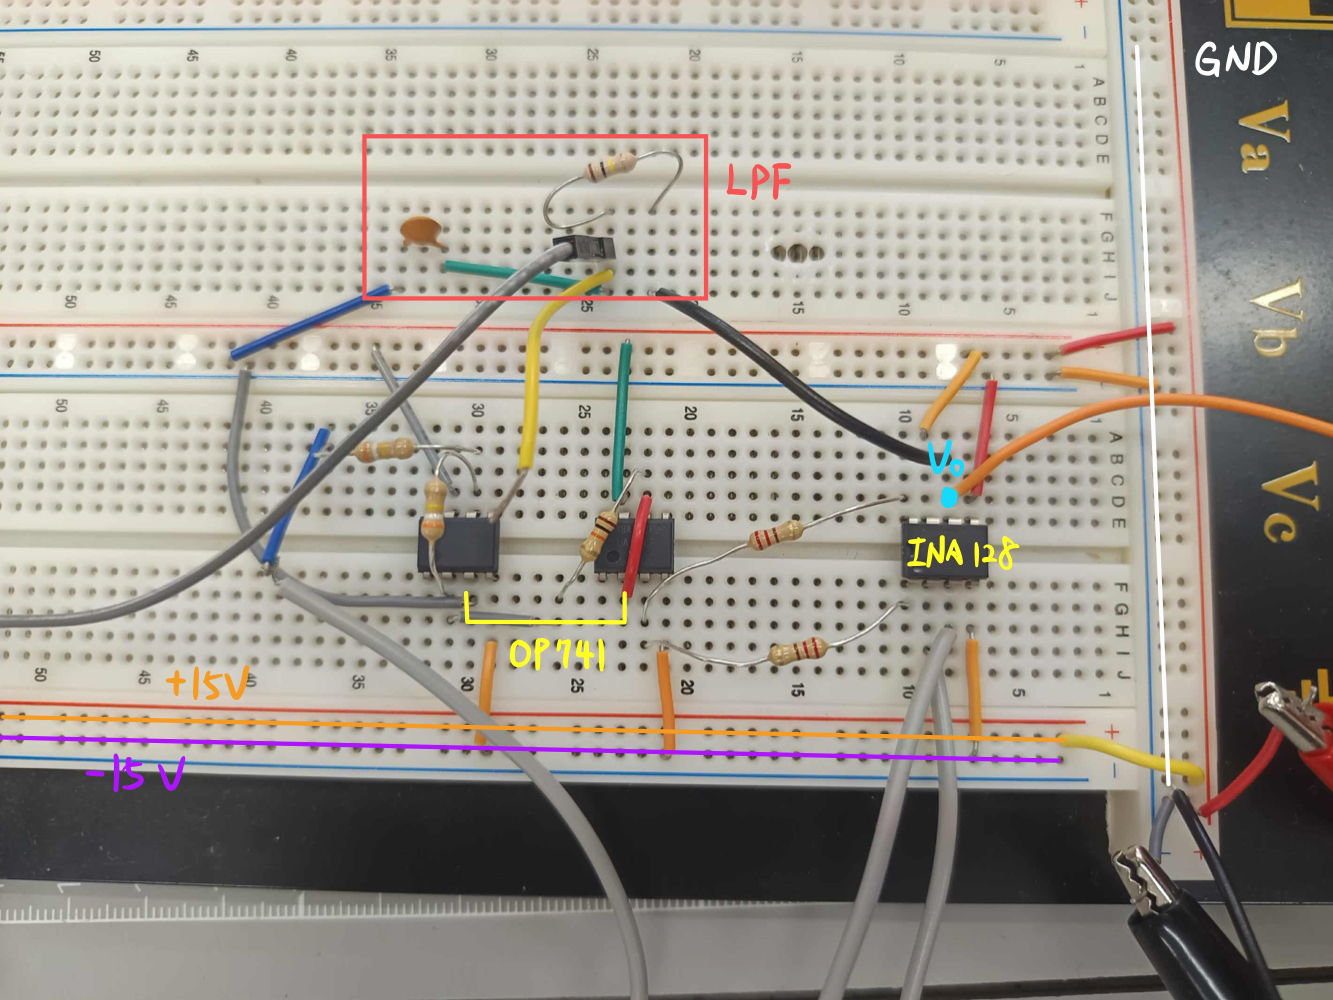
\includegraphics[width=0.8\linewidth]{fig/electric_design.jpg}
    \caption{Circuit design}
    \label{fig:elec}
\end{figure}
%%%%%%%%%%%%%%%%%%%%%%%%%%%%%%%%%%%%%%%%%%%%%%%%%%%%%%%%%%%%%%%%%%
\section{Frequency and Gain Characterization of the INA}
%%%%%%%%%%%%%%%%%%%%%%%%%%%%%%%%%%%%%%%%%%%%%%%%%%%%%%%%%%%%%%%%%%



\subsection{Output Amplitude versus $R_G$}

Figure~\ref{fig:vout_rg} shows the measured output amplitude $V_{\text{out}}$ as a function of the gain-setting resistor $R_G$, with the theoretical prediction overlaid. The trend follows the standard instrumentation amplifier relationship:
\begin{equation}
    G = 1 + \frac{50~\text{k}\Omega}{R_G}.
\end{equation}
As expected, smaller $R_G$ values yield higher gain and therefore larger $V_{\text{out}}$ at a fixed input amplitude of $V_{\text{in}} = 20~\text{mV}_{\text{pp}}$.

Using this model, the predicted output amplitudes are approximately 
\[
V_{\text{out}} \approx 
\begin{cases}
121~\text{mV}_{\text{pp}}, & R_G = 9.9~\text{k}\Omega~(G \approx 6.05)\\
220~\text{mV}_{\text{pp}}, & R_G = 5.0~\text{k}\Omega~(G = 11)\\
1.01~\text{V}_{\text{pp}}, & R_G = 1.011~\text{k}\Omega~(G \approx 50.5)
\end{cases}
\]
The corresponding measurements were $150$, $245$, and $1.00~\text{V}_{\text{pp}}$, respectively. The high-gain point agrees with theory within $\sim 1\%$, while the lower-gain points are roughly $11\text{–}24\%$ higher than predicted. 

This discrepancy pattern is typical when the measurement setup dominates the total error: small inaccuracies in the function generator amplitude or probe attenuation translate directly into apparent gain deviations. In addition, $R_G$ tolerance and input-offset/CMR effects are more pronounced at lower gains. Importantly, the overall linear dependence of $V_{\text{out}}$ on $R_G$ confirms that the amplifier operates linearly near $100~\text{Hz}$, so a narrow input pulse should be faithfully amplified by the expected gain $G$ without compression in this regime.

Our final choice for $R_G$ in the later experiment is $110\Omega$ as our observed $R_G$ sweep suggested a lower resistance for better amplification.
\begin{figure}[H]
    \centering
    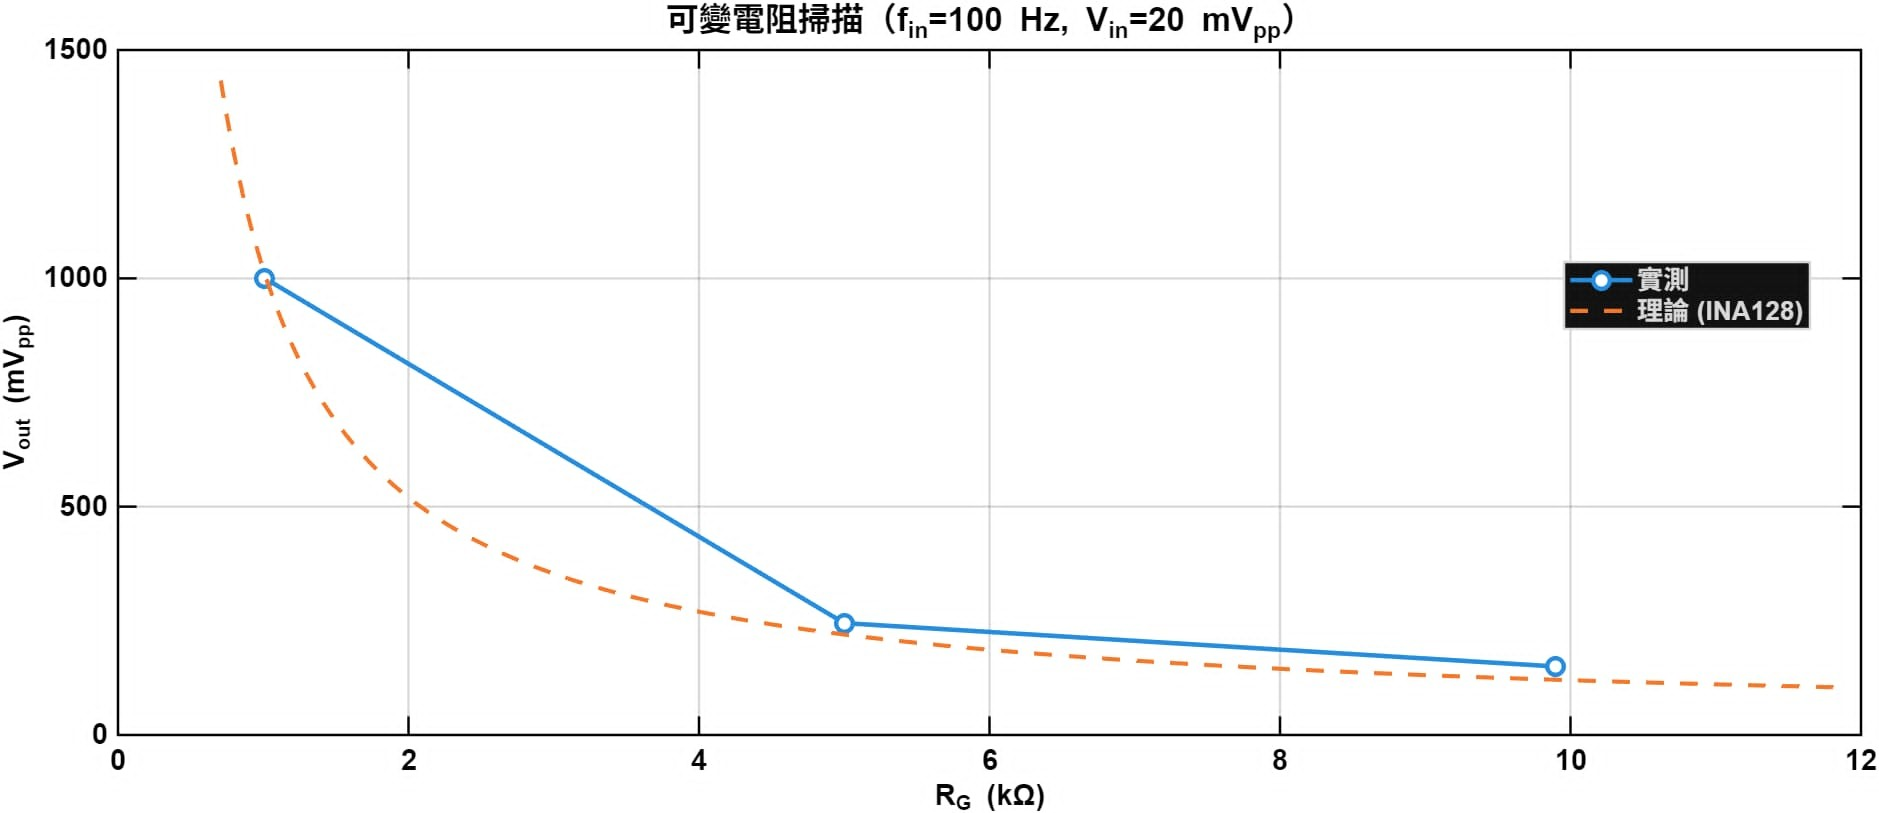
\includegraphics[width=0.8\linewidth]{fig/vout_rg.jpg}
    \caption{$V_{\text{out}}$ vs.\ $R_G$ with theoretical gain model overlaid.}
    \label{fig:vout_rg}
\end{figure}


\subsection{Frequency Response}

Figure~\ref{fig:freq_sweep} shows the frequency sweep for $R_G \approx 9.9~\text{k}\Omega$. The output remains approximately $150~\text{mV}_{\text{pp}}$ from $1$ to $100~\text{Hz}$ and decreases gently to $121~\text{mV}_{\text{pp}}$ at $100~\text{kHz}$, corresponding to a $\approx -1.86~\text{dB}$ drop relative to $1~\text{Hz}$. 

For an instrumentation amplifier configured with $G \approx 6$, the small-signal $-3~\text{dB}$ bandwidth is expected to lie well above $100~\text{kHz}$, so this modest droop is reasonable and likely due to the external setup (generator amplitude roll-off, probe loading, or input stray capacitance) rather than the amplifier itself. The required slew rate at $100~\text{kHz}$ and $150~\text{mV}_{\text{pp}}$ is
\begin{equation}
    \frac{dV}{dt}_{\max} = 2\pi f V_{\text{peak}} \approx 0.047~\text{V}/\mu\text{s},
\end{equation}
which is far below the typical $1~\text{V}/\mu\text{s}$ capability of the device, confirming that slew-rate limitation is not a concern.

Since we know our signal would be at low frequency, the amplifier behaves completely feasible.

\begin{figure}[H]
    \centering
    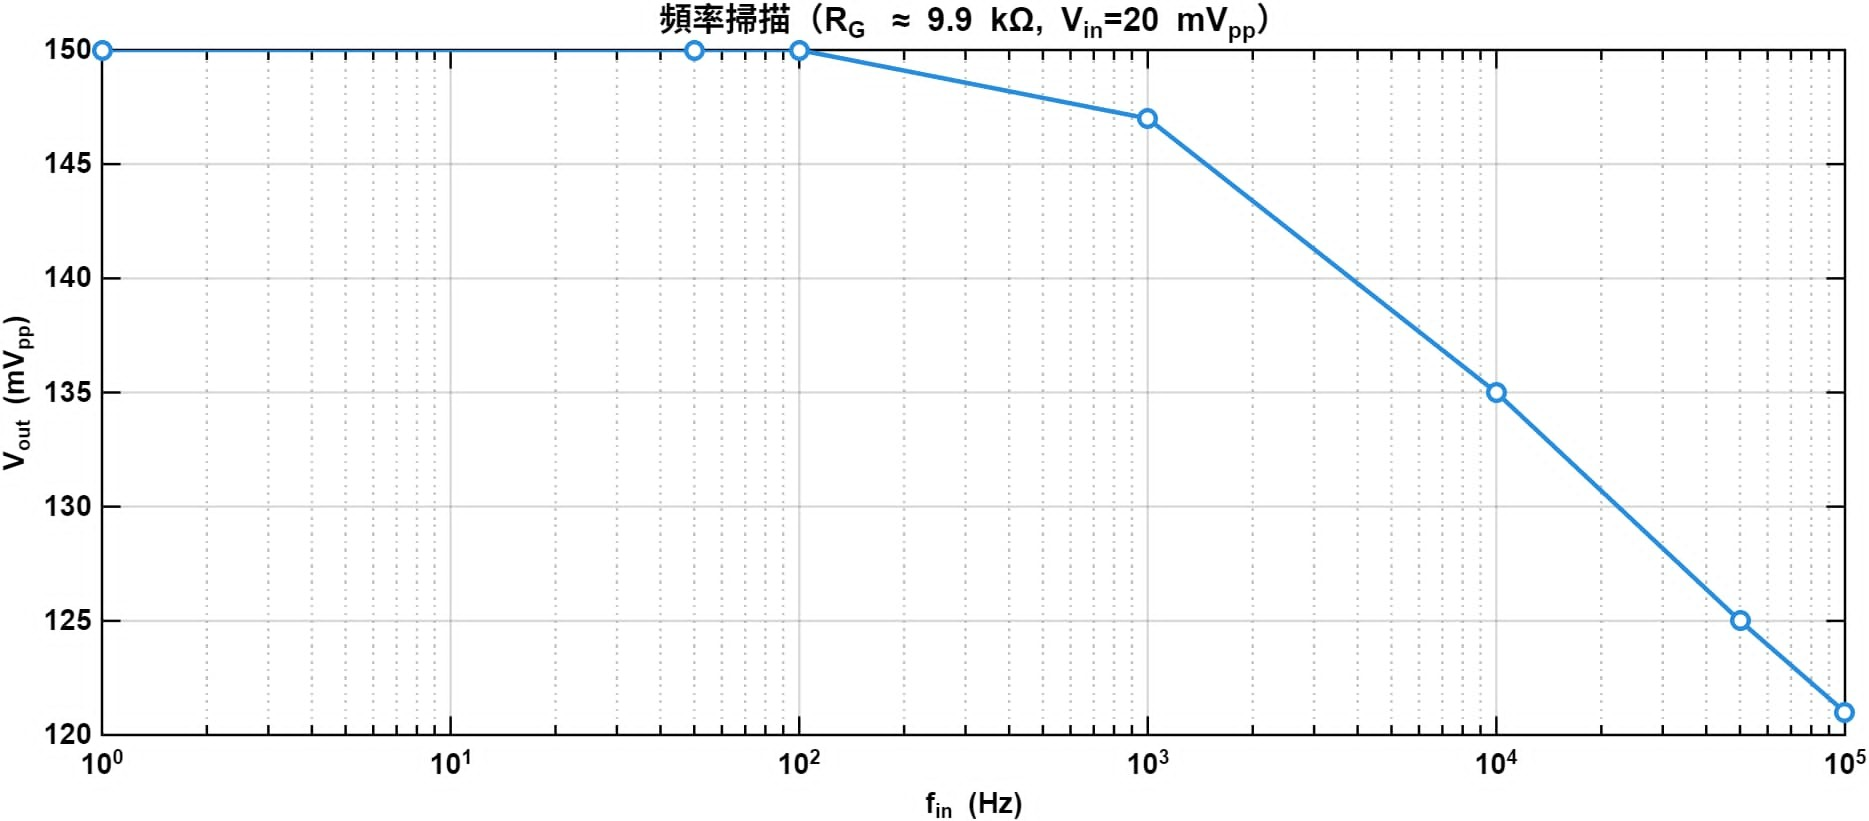
\includegraphics[width=0.8\linewidth]{fig/freq_sweep.jpg}
    \caption{Frequency response for $R_G \approx 9.9~\text{k}\Omega$ ($G \approx 6$).}
    \label{fig:freq_sweep}
\end{figure}


%%%%%%%%%%%%%%%%%%%%%%%%%%%%%%%%%%%%%%%%%%%%%%%%%%%%%%%%%%%%%%%%%%
\section{Signal Processing}
%%%%%%%%%%%%%%%%%%%%%%%%%%%%%%%%%%%%%%%%%%%%%%%%%%%%%%%%%%%%%%%%%%

\subsection{Direct Digital Filtering on Oversampled Signal}

The first attempt of our signal processing was to design a direct filtering on the oversampled signal. The basic structures were concluded by the following block diagram.

We targeted on retaining the desired signal around $0.7\sim 30$Hz, and focusing on filtering out the known 60Hz noise from the power cord.
\begin{figure}[h]
  \centering
  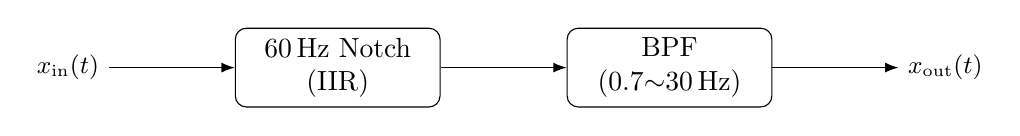
\begin{tikzpicture}[node distance=1.6cm]
    \node[io]    (in)   {$x_\text{in}(t)$};
    \node[block, right=of in]   (notch) {60\,Hz Notch\\(IIR)};
    \node[block, right=of notch] (lpf)  {BPF\\(0.7$\sim$30\,Hz)};
    \node[io, right=of lpf]      (out)    {$x_\text{out}(t)$};

    \draw[->] (in) -- (notch);
    \draw[->] (notch) -- (lpf);
    \draw[->] (lpf) -- (out);
  \end{tikzpicture}
  \caption{Direct digital processing with the oversampled signal}
  \label{tikz:os_sig_pipe}
\end{figure}

\paragraph{Implementations and results}
We design the following parts: we first notch down the 60Hz noise peak, and then pass the signal through a bandpass filter.  
\begin{lstlisting}[caption={Baseline and 60 Hz cleanup with bandpass filtering.}, label={lst:ecg_filter}]
%% ===================== 1) 60 Hz notch ======================
notch60 = designfilt('bandstopiir','FilterOrder',2, ...
    'HalfPowerFrequency1',56,'HalfPowerFrequency2',57, ...
    'DesignMethod','butter','SampleRate',Fs);

%% ===================== 2) Bandpass 0.7~30 Hz ============================
bp = designfilt('bandpassiir','FilterOrder',6, ...
    'HalfPowerFrequency1',0.7,'HalfPowerFrequency2',30, ...
    'DesignMethod','butter','SampleRate',Fs);
\end{lstlisting}

We observe the filtered signal with the orignal signal (Blue) at different stages(Orange and Yellow). We can see that with the 60Hz notch we can effectively lower the noise from 55.7dB to 4.01dB.

\begin{figure}[H]
	\centering 
		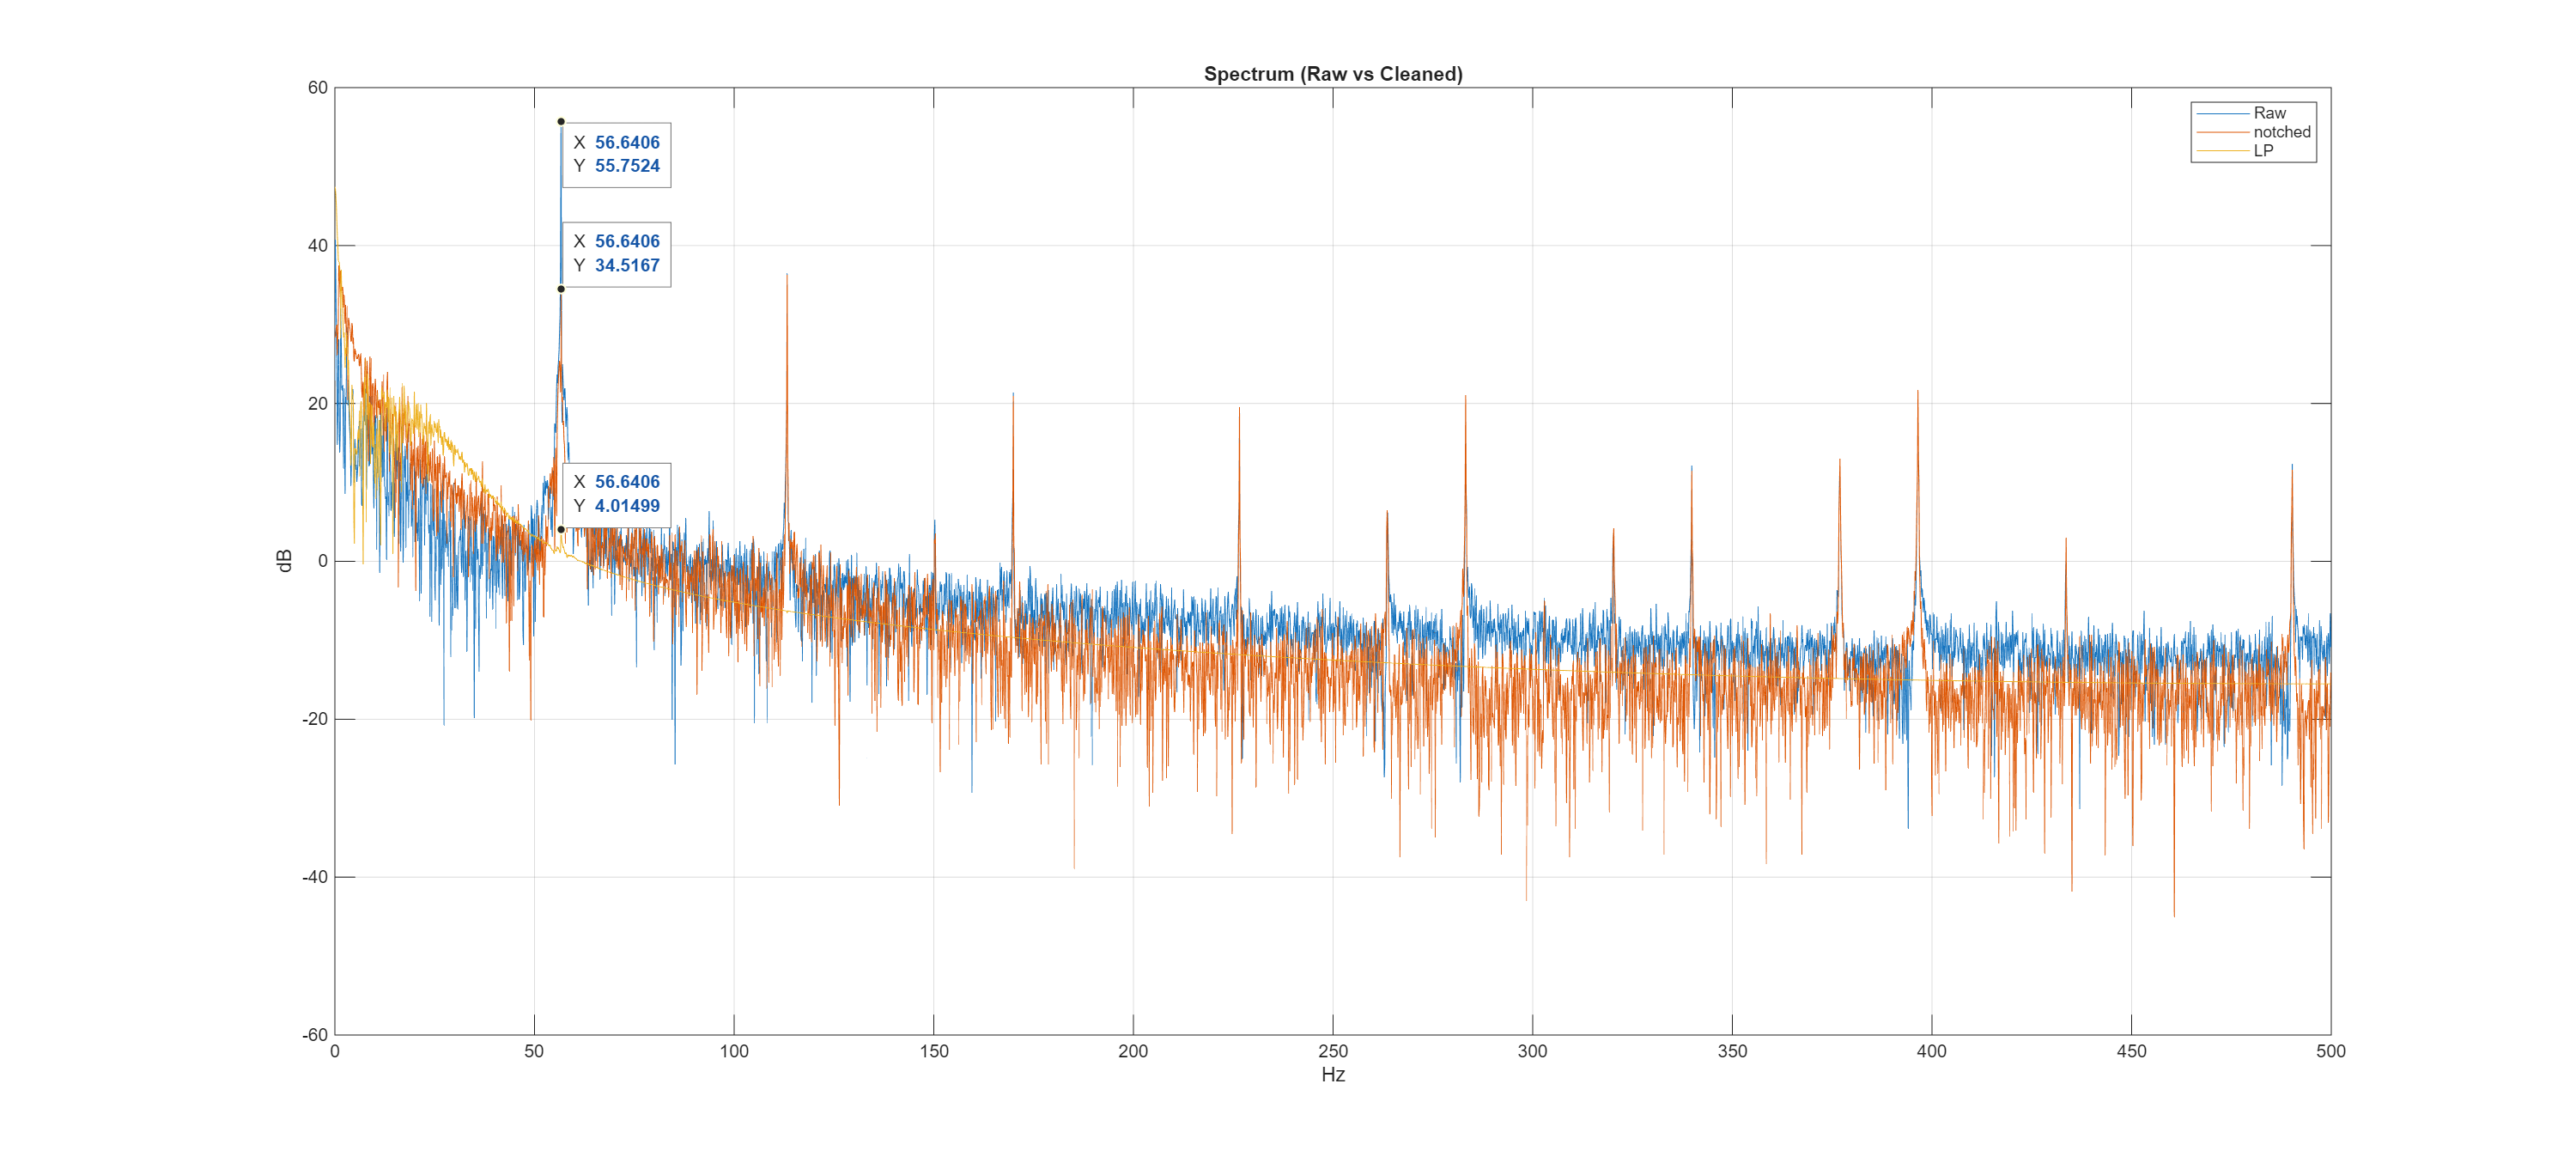
\includegraphics[width = .95\columnwidth]{fig/freq_direct_filt.png}
	\caption{Direct DSP techniques on the oversampled signal in frequency domain}
\label{fig:os_freq}
\end{figure}

The filtered signal is already pretty ideal.

\begin{figure}[H]
	\centering 
		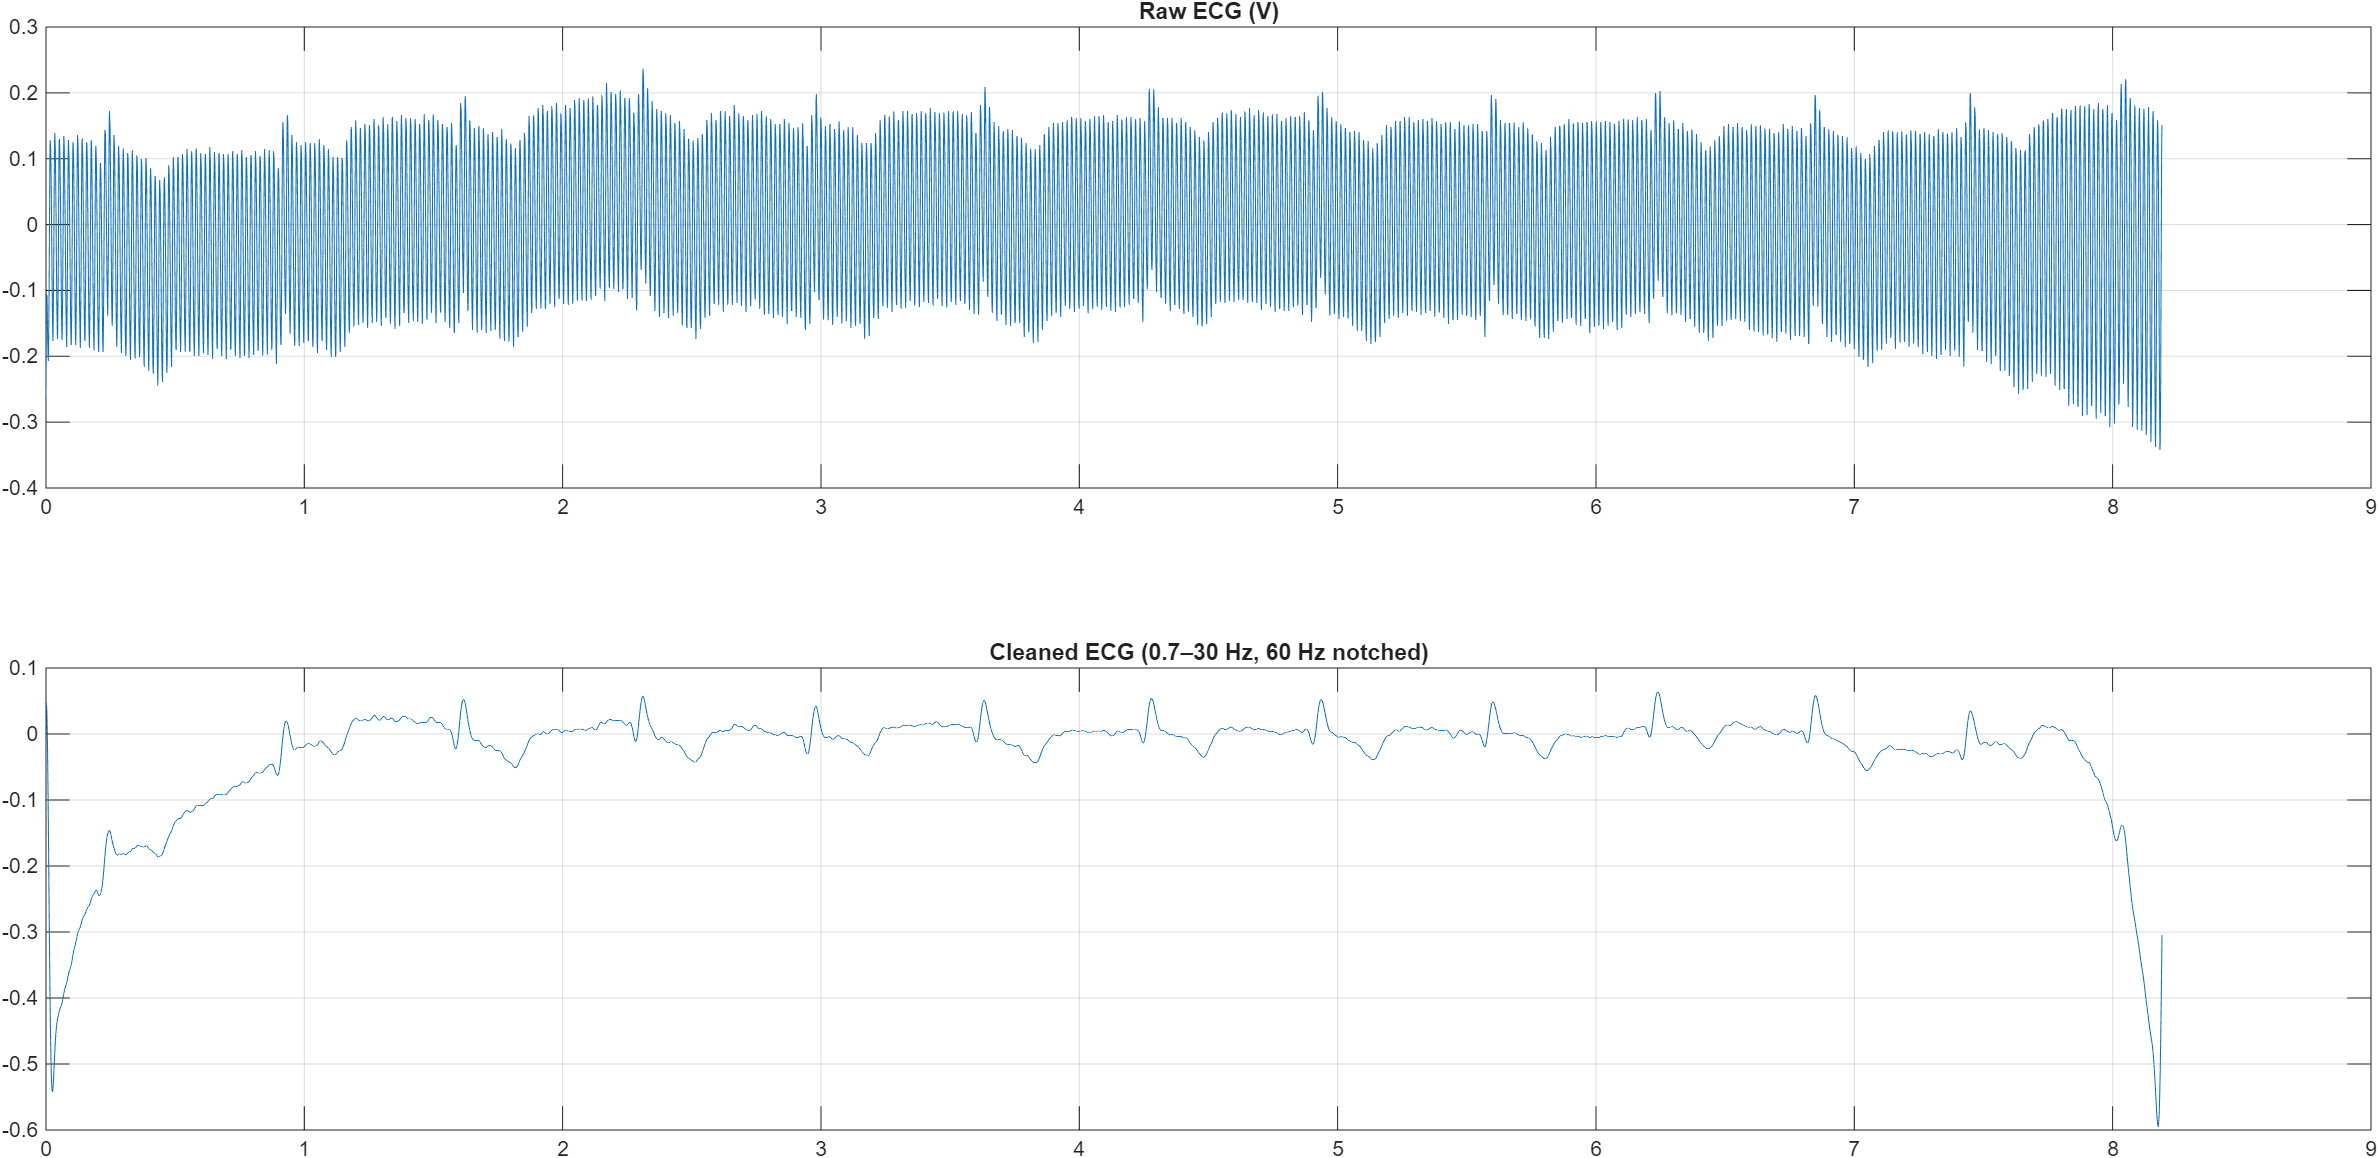
\includegraphics[width = .95\columnwidth]{fig/time_origin_filt.png}
	\caption{Direct DSP techniques on the oversampled signal in time domain}
\label{fig:os_time_cmp}
\end{figure}

This is the first time we deal with natural source signals. We try to discuss about some interesting things we've found out in this part.

\paragraph{Distortion at the Beginning and End of the IIR-filtered Signal.}

In the reconstructed ECG signal we can observe an obious distortion at the head and tail of the signals. 
In the implementation we're already using \lstinline|filtfilt()|, so the forward and backward filtering should already eliminate the zero phase distortion.

This is caused by the narrowband filter we're using in the DSP process. The DC removal filter was designed to be a 0.7Hz highpass iir filter, which naturally has a long time constants ($1/0.7 \sim 1.43s$). 
The abrupted signals at the start and end makes the mirrored signal not so much continuous, hence the settling lasts long enough to distord the signal. If we pull out the DC remover we can observe a smoother pattern.
\begin{figure}[H]
	\centering 
		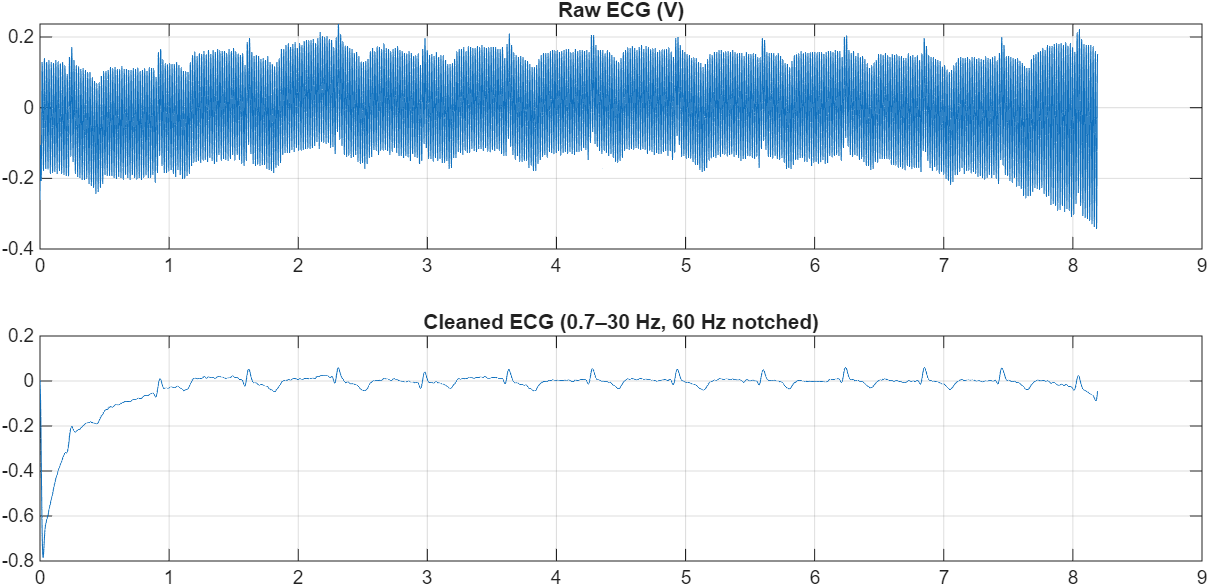
\includegraphics[width = .95\columnwidth]{fig/time_origin_filt_nohp.png}
	\caption{Signals with no DC removal narrowband filter}
\label{fig:os_time_cmp_nohp}
\end{figure}

\paragraph{Harmonic Series of noise.}
In addition to the 60 Hz fundamental noise, the spectrum exhibits harmonics at integer multiples of 60 Hz. These arise from nonlinear coupling and rectification of power-line interference in the measurement electronics. The smaller peaks surrounding each harmonic are modulation or spectral-leakage sidebands caused by the interaction between power-line hum and the ECG baseline or by slight frequency mismatch with the FFT window.

\subsection{Downsampling}

With this basic filtering structure we proceed with our main dish in the experiment this time.

Our choice of the downsampling rate was $M=4$ as in the example gave out in the slides, while in theory since our desired signal is known to be lower than $30$Hz, 
the theoretical feasible downsampling rate is $\frac{F_s}{2f_\text{BW}} = 1000/60 \simeq 16.6$.

\begin{figure}[h]
  \centering
  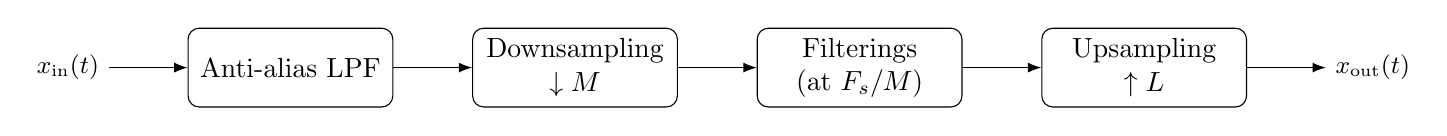
\begin{tikzpicture}[node distance=1.0cm]
    \node[io]    (in)   {$x_\text{in}(t)$};
    \node[block, right=of in]   (aa)     {Anti-alias LPF};
    \node[block, right=of aa]   (ds)     {Downsampling\\$\downarrow M$};
    \node[block, right=of ds]   (post)   {Filterings\\(at $F_s/M$)};
    \node[block, right=of post] (us)     {Upsampling\\$\uparrow L$};
    \node[io, right=of us]      (out)    {$x_\text{out}(t)$};

    \draw[->] (in) -- (aa);
    \draw[->] (aa) -- (ds);
    \draw[->] (ds) -- (post);
    \draw[->] (post) -- (us);
    \draw[->] (us) -- (out);
  \end{tikzpicture}
  \caption{Signal Processing Pipeline with Downsampling} 
  \label{tikz:ds_sig_pipe}
\end{figure}

\begin{lstlisting}[caption={Anti-alias low-pass filtering before downsampling.}, label={lst:aa_filter}]
aa = designfilt('lowpassiir','FilterOrder',8, ...
    'HalfPowerFrequency', 0.9*(Fs_ds/2), ...
    'DesignMethod','butter','SampleRate',Fs);
x_aa = filtfilt(aa, x);
\end{lstlisting}

We can see, as in our digital signal processing lectures suggested, the downsapling in time domain gives us a stretch in the frequency domain. 
\begin{figure}[H]
	\centering 
		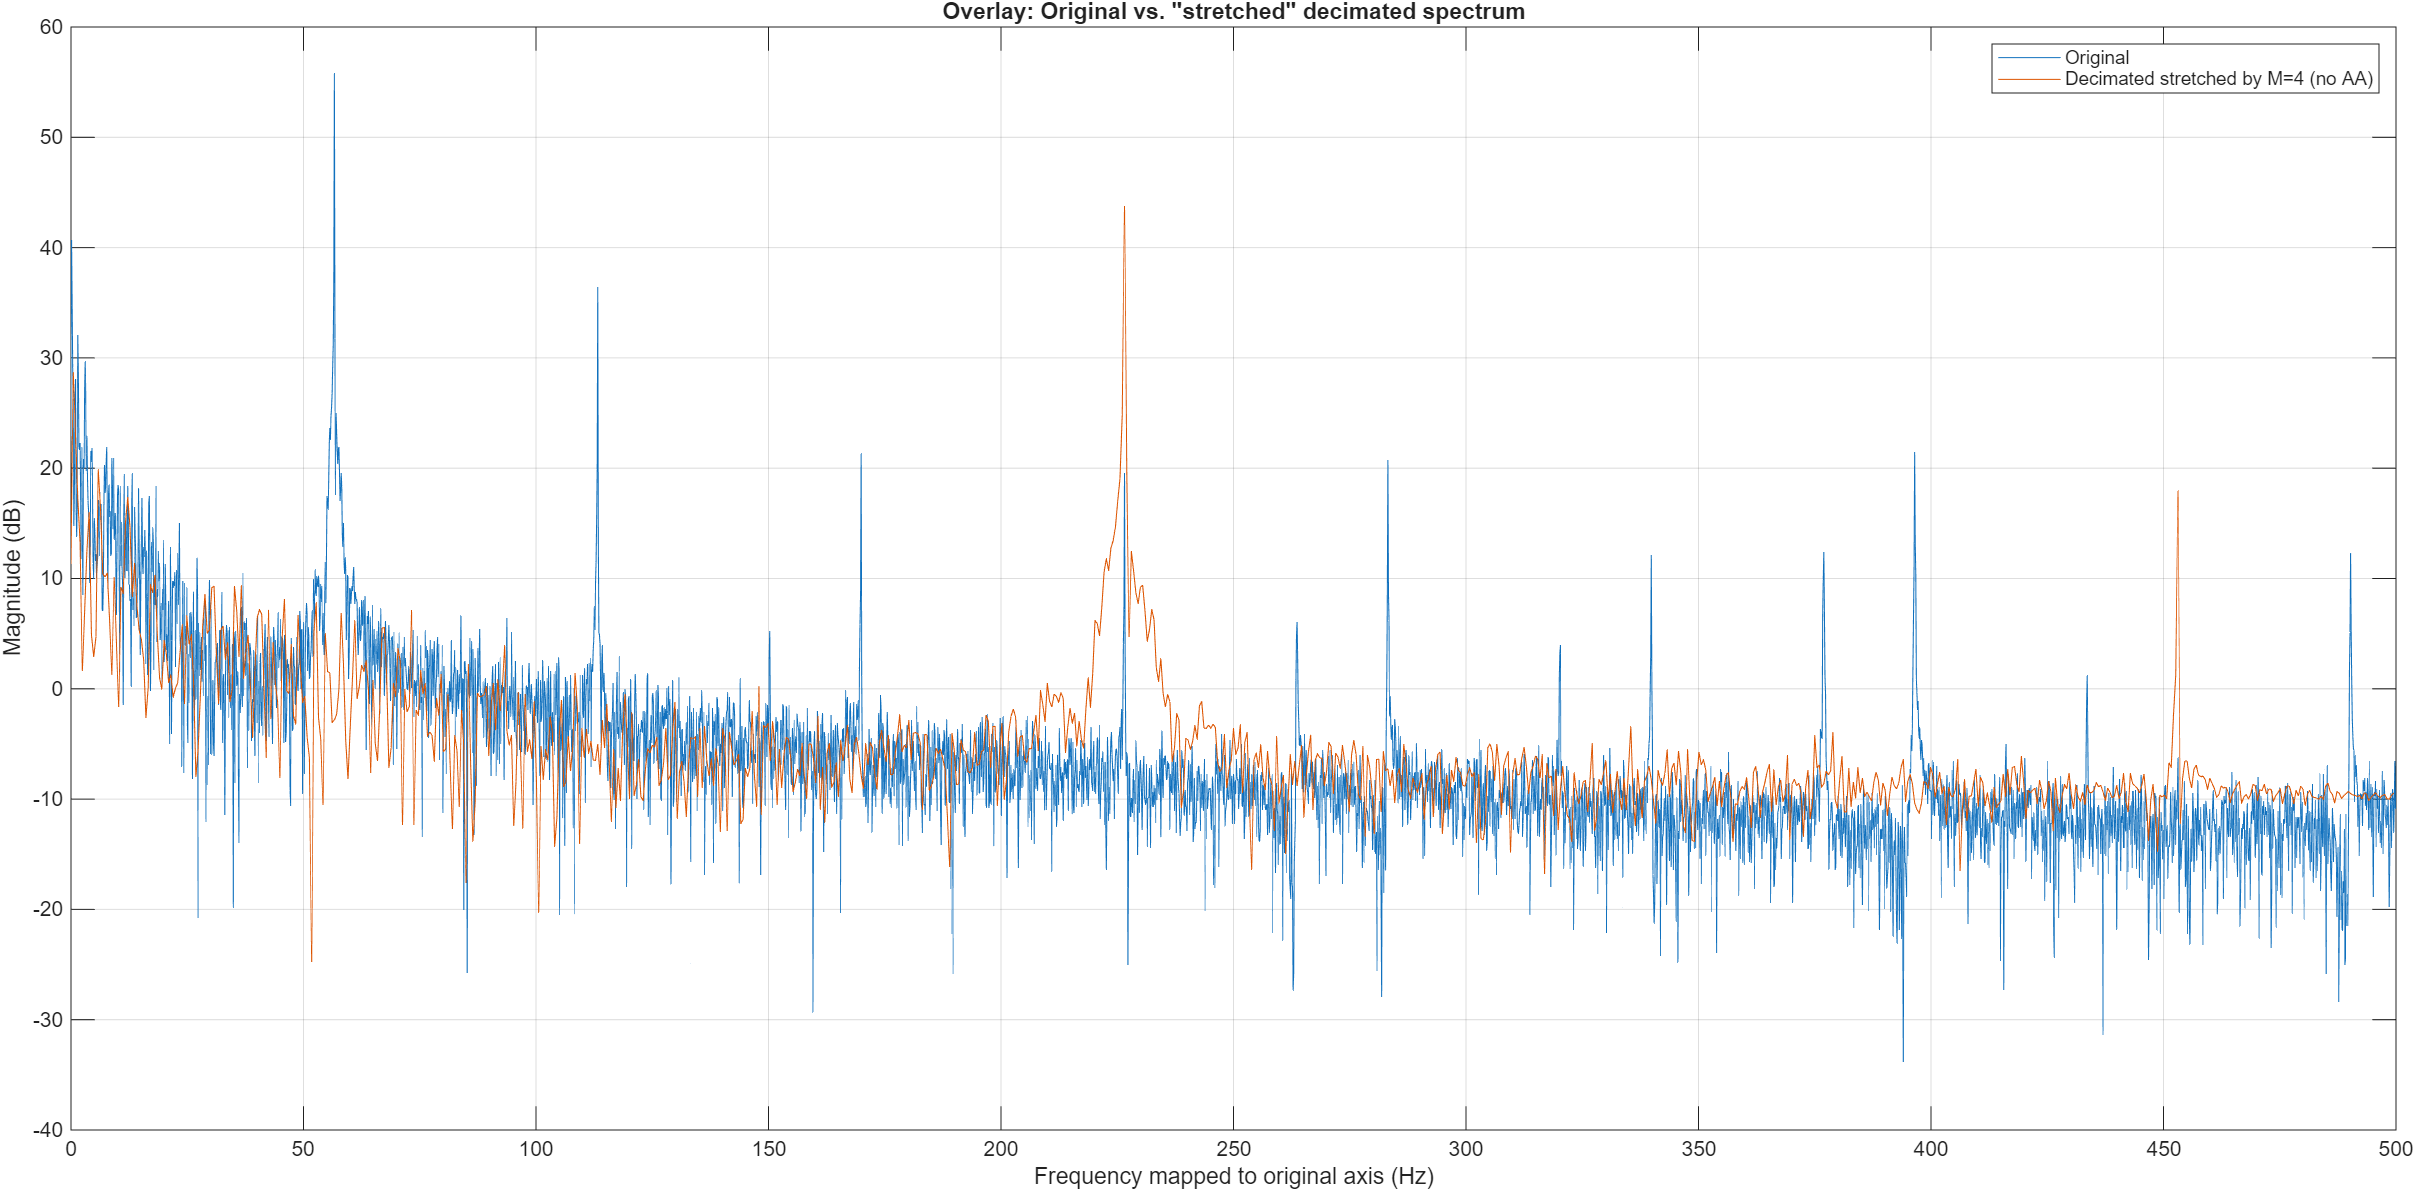
\includegraphics[width = .95\columnwidth]{fig/freq_downsamp_origin_cmp.png}
	\caption{}
\label{fig:freq_ds_os_cmp}
\end{figure}

\begin{lstlisting}[caption={Direct and averaged downsampling.}, label={lst:downsample}]
% Direct downsampling
x_ds = x_aa(1:M:end);
t_ds = t(1:M:end);

% Averaged downsampling
Lfull     = floor(numel(x)/M)*M;
x_trunc   = x_aa(1:Lfull);
x_blocks  = reshape(x_trunc, M, []);
x_ds_avg  = mean(x_blocks,1).';
\end{lstlisting}



We then apply the same filtering design on the downsampled signal.
\begin{lstlisting}[caption={High-pass, notch, and band-pass filtering at the reduced sampling rate.}, label={lst:downsample_filter}]
hp_ds = designfilt('highpassiir','FilterOrder',4, ...
    'HalfPowerFrequency',0.7,'SampleRate',Fs_ds,'DesignMethod','butter');
bp_ds = designfilt('bandpassiir','FilterOrder',6, ...
    'HalfPowerFrequency1',0.7,'HalfPowerFrequency2',30, ...
    'DesignMethod','butter','SampleRate',Fs_ds);
notch_ds = designfilt('bandstopiir','FilterOrder',2, ...
    'HalfPowerFrequency1',56,'HalfPowerFrequency2',57, ...
    'DesignMethod','butter','SampleRate',Fs_ds);

x_ds_hp  = filtfilt(hp_ds,   x_ds);
x_ds_n60 = filtfilt(notch_ds, x_ds_hp);
x_ds_bp  = filtfilt(bp_ds,   x_ds_n60);

x_ds_hp_avg  = filtfilt(hp_ds,   x_ds_avg);
x_ds_n60_avg = filtfilt(notch_ds, x_ds_hp_avg);
x_ds_bp_avg  = filtfilt(bp_ds,   x_ds_n60_avg);
\end{lstlisting}

\begin{lstlisting}[caption={Reconstructing the signal to 1 kHz via interpolation.}, label={lst:upsample}]
x_up      = interp1(t_ds, x_ds_bp, t_trim, 'pchip', 'extrap');
x_up_avg  = interp1(t_ds, x_ds_bp_avg, t_trim, 'pchip', 'extrap');
\end{lstlisting}

We can see an obvious difference on the ambient noise level. (with the normalized frequency axis by $F_s/M$). This is much more obvious if we increase our downsample rate to $M=8$
The figures on the left show $M=4$, right show $M=8$.

\begin{figure}[H]
	\centering 
	\subcaptionbox{\centering $M=4$ 
		\label{fig:freq_down_M4}}{
		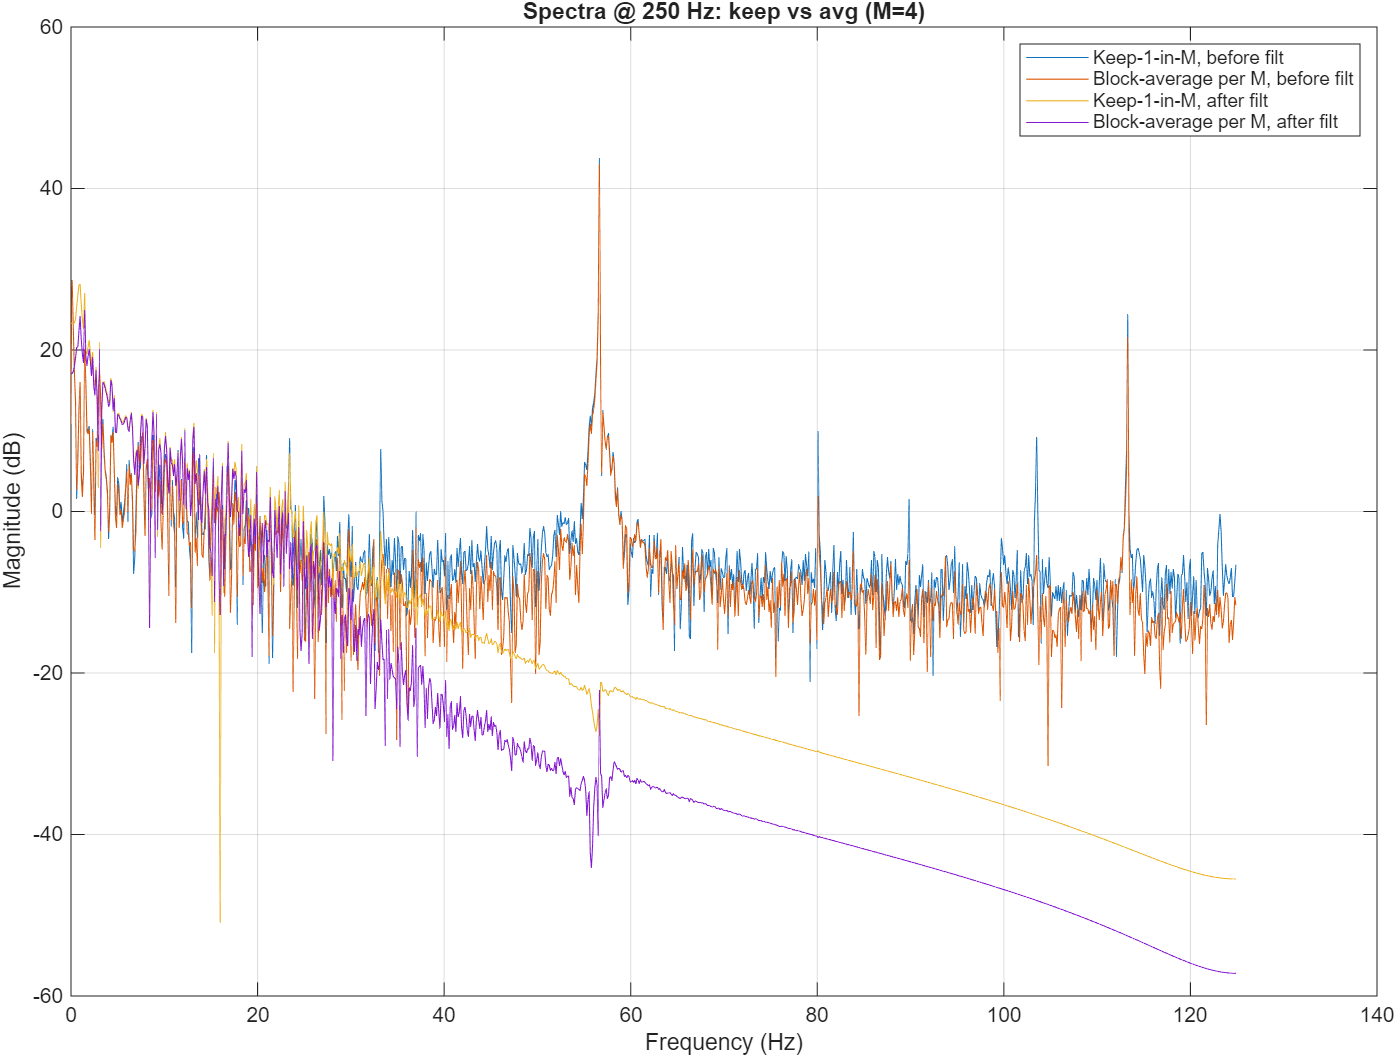
\includegraphics[height= .25\columnwidth]{fig/freq_downsamp_filt.png}
    }
	\subcaptionbox{\centering $M=8$
		\label{fig:freq_down_M8}}{
		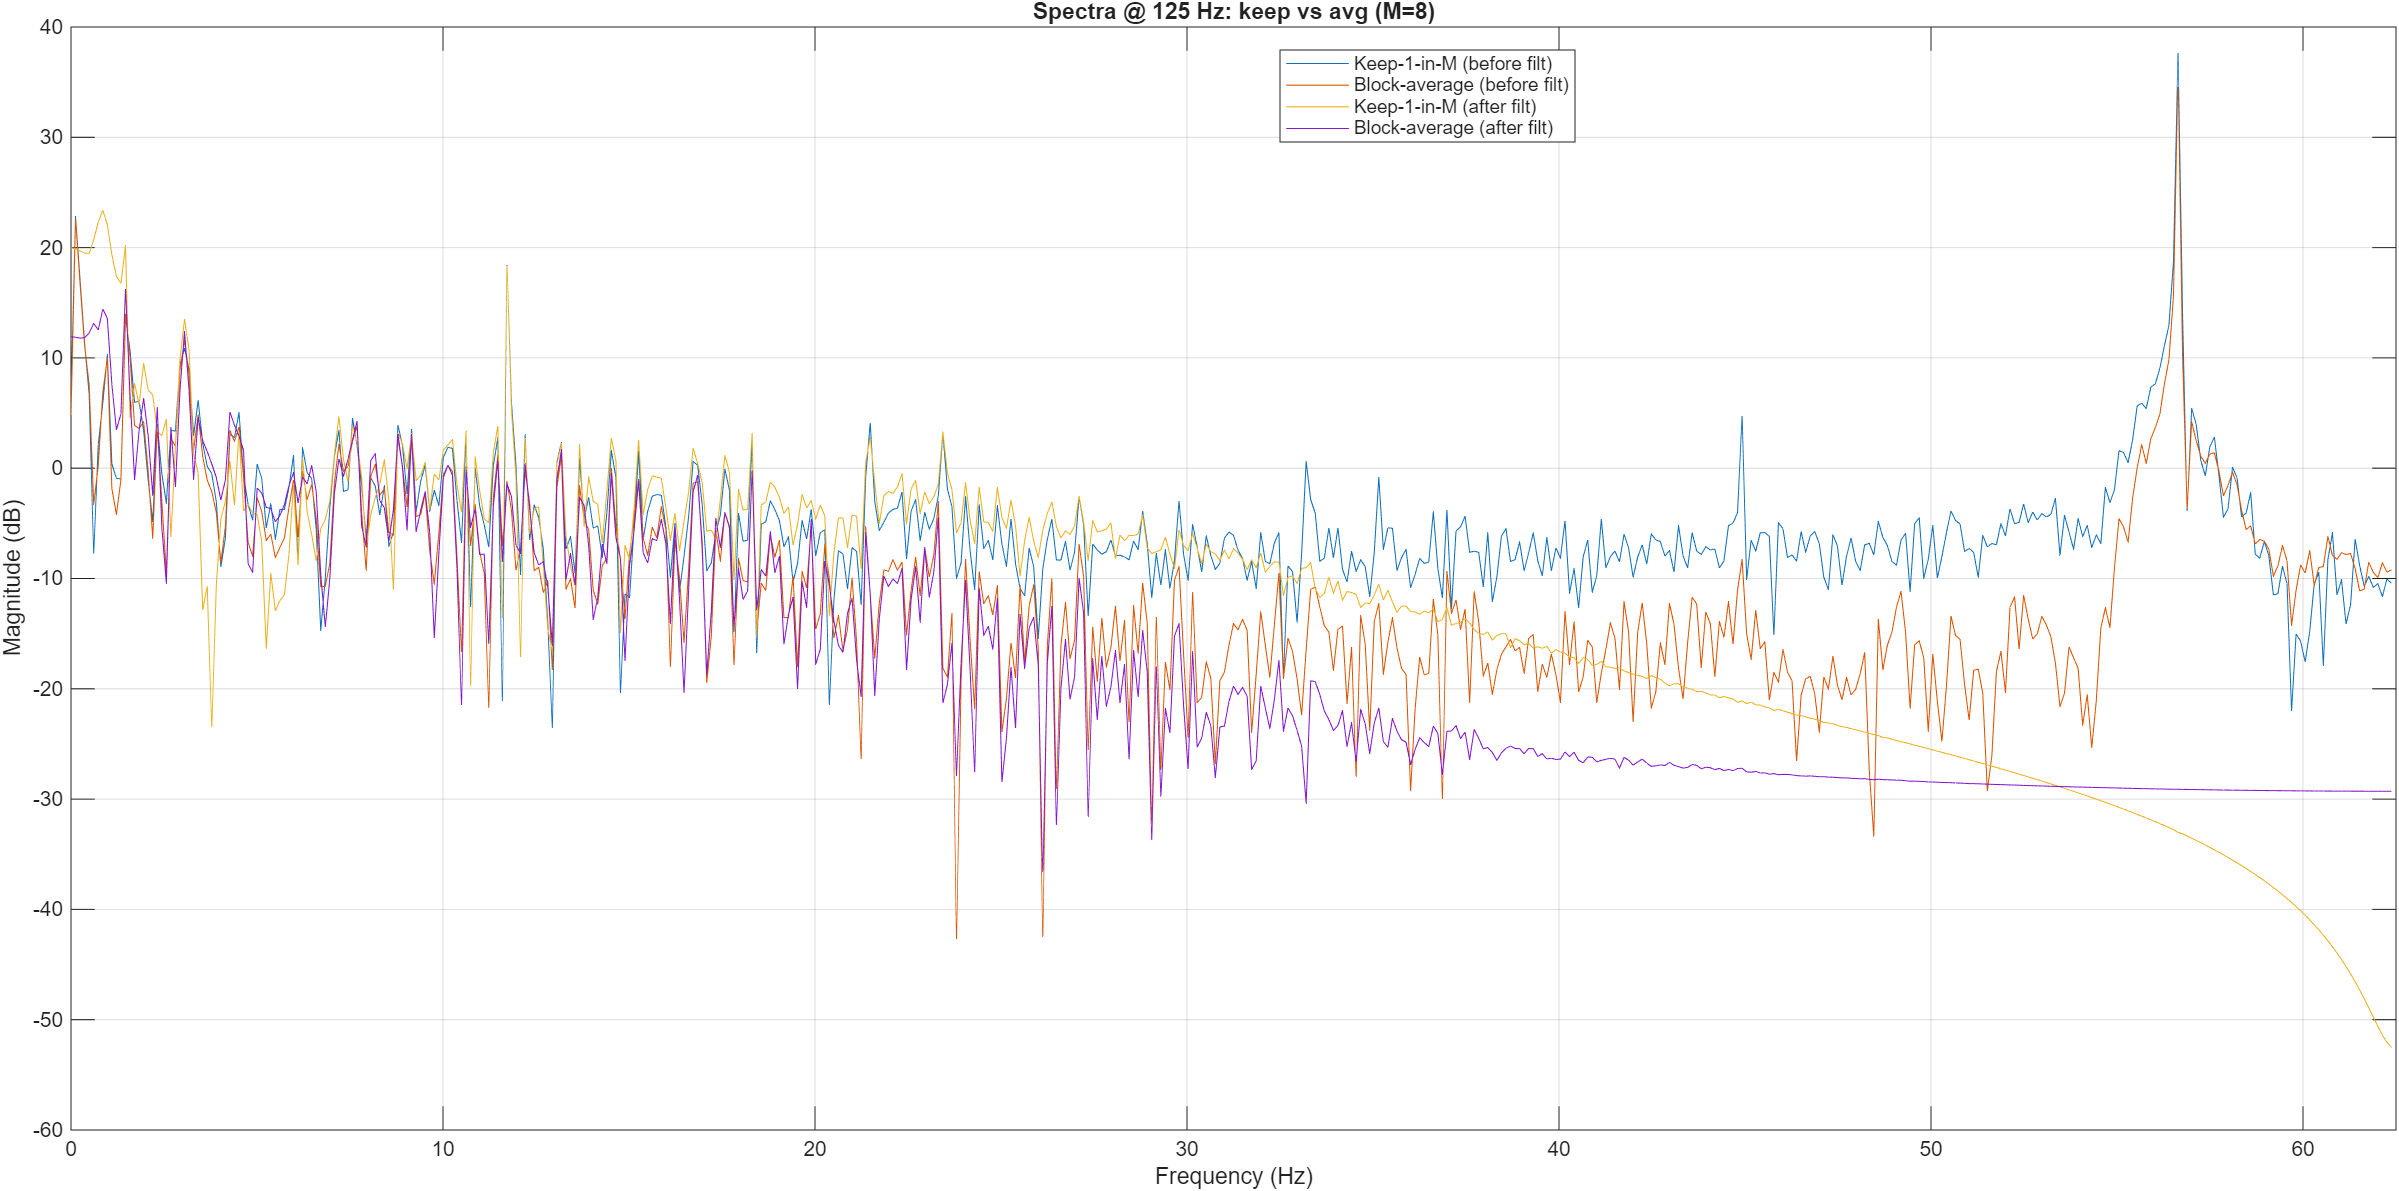
\includegraphics[height= .25\columnwidth]{fig/freq_downsamp_filt_M8.png}
    }
  \caption{Frequency domain signal comparison of the two downsampling techniques, before and after filtering}
\label{fig:ds_freq_filt}
\end{figure}

\begin{figure}[H]
	\centering 
	\subcaptionbox{\centering $M=4$ 
		\label{fig:time_down_M4}}{
		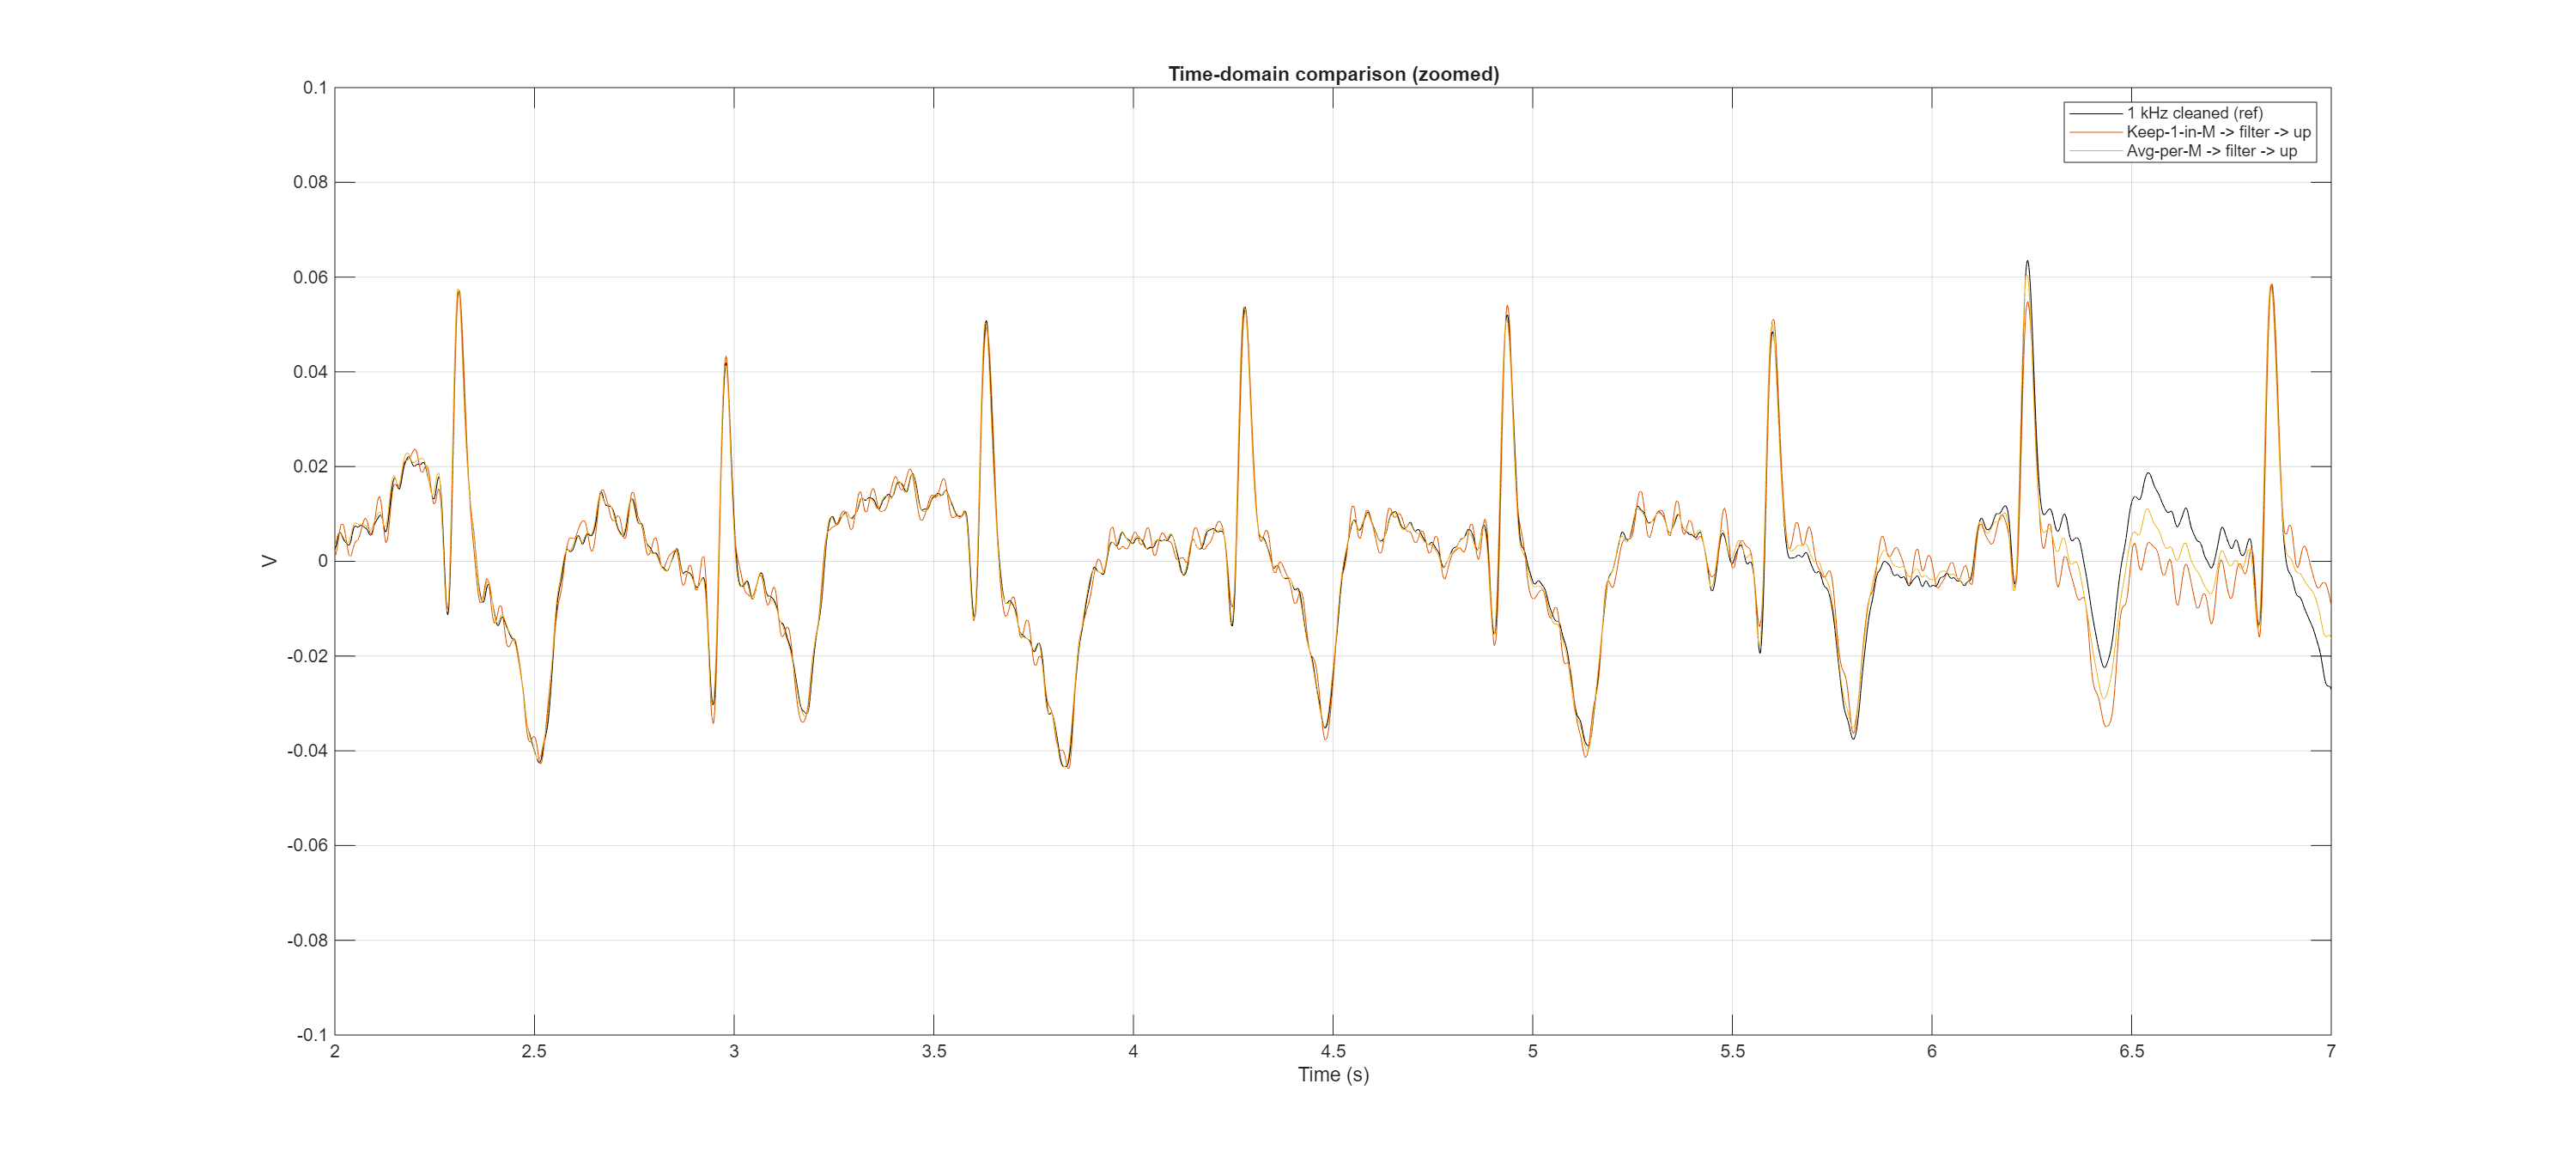
\includegraphics[width= .9\columnwidth]{fig/time_downsamp_zoom.png}
    }
	\subcaptionbox{\centering $M=8$
		\label{fig:time_down_M8}}{
		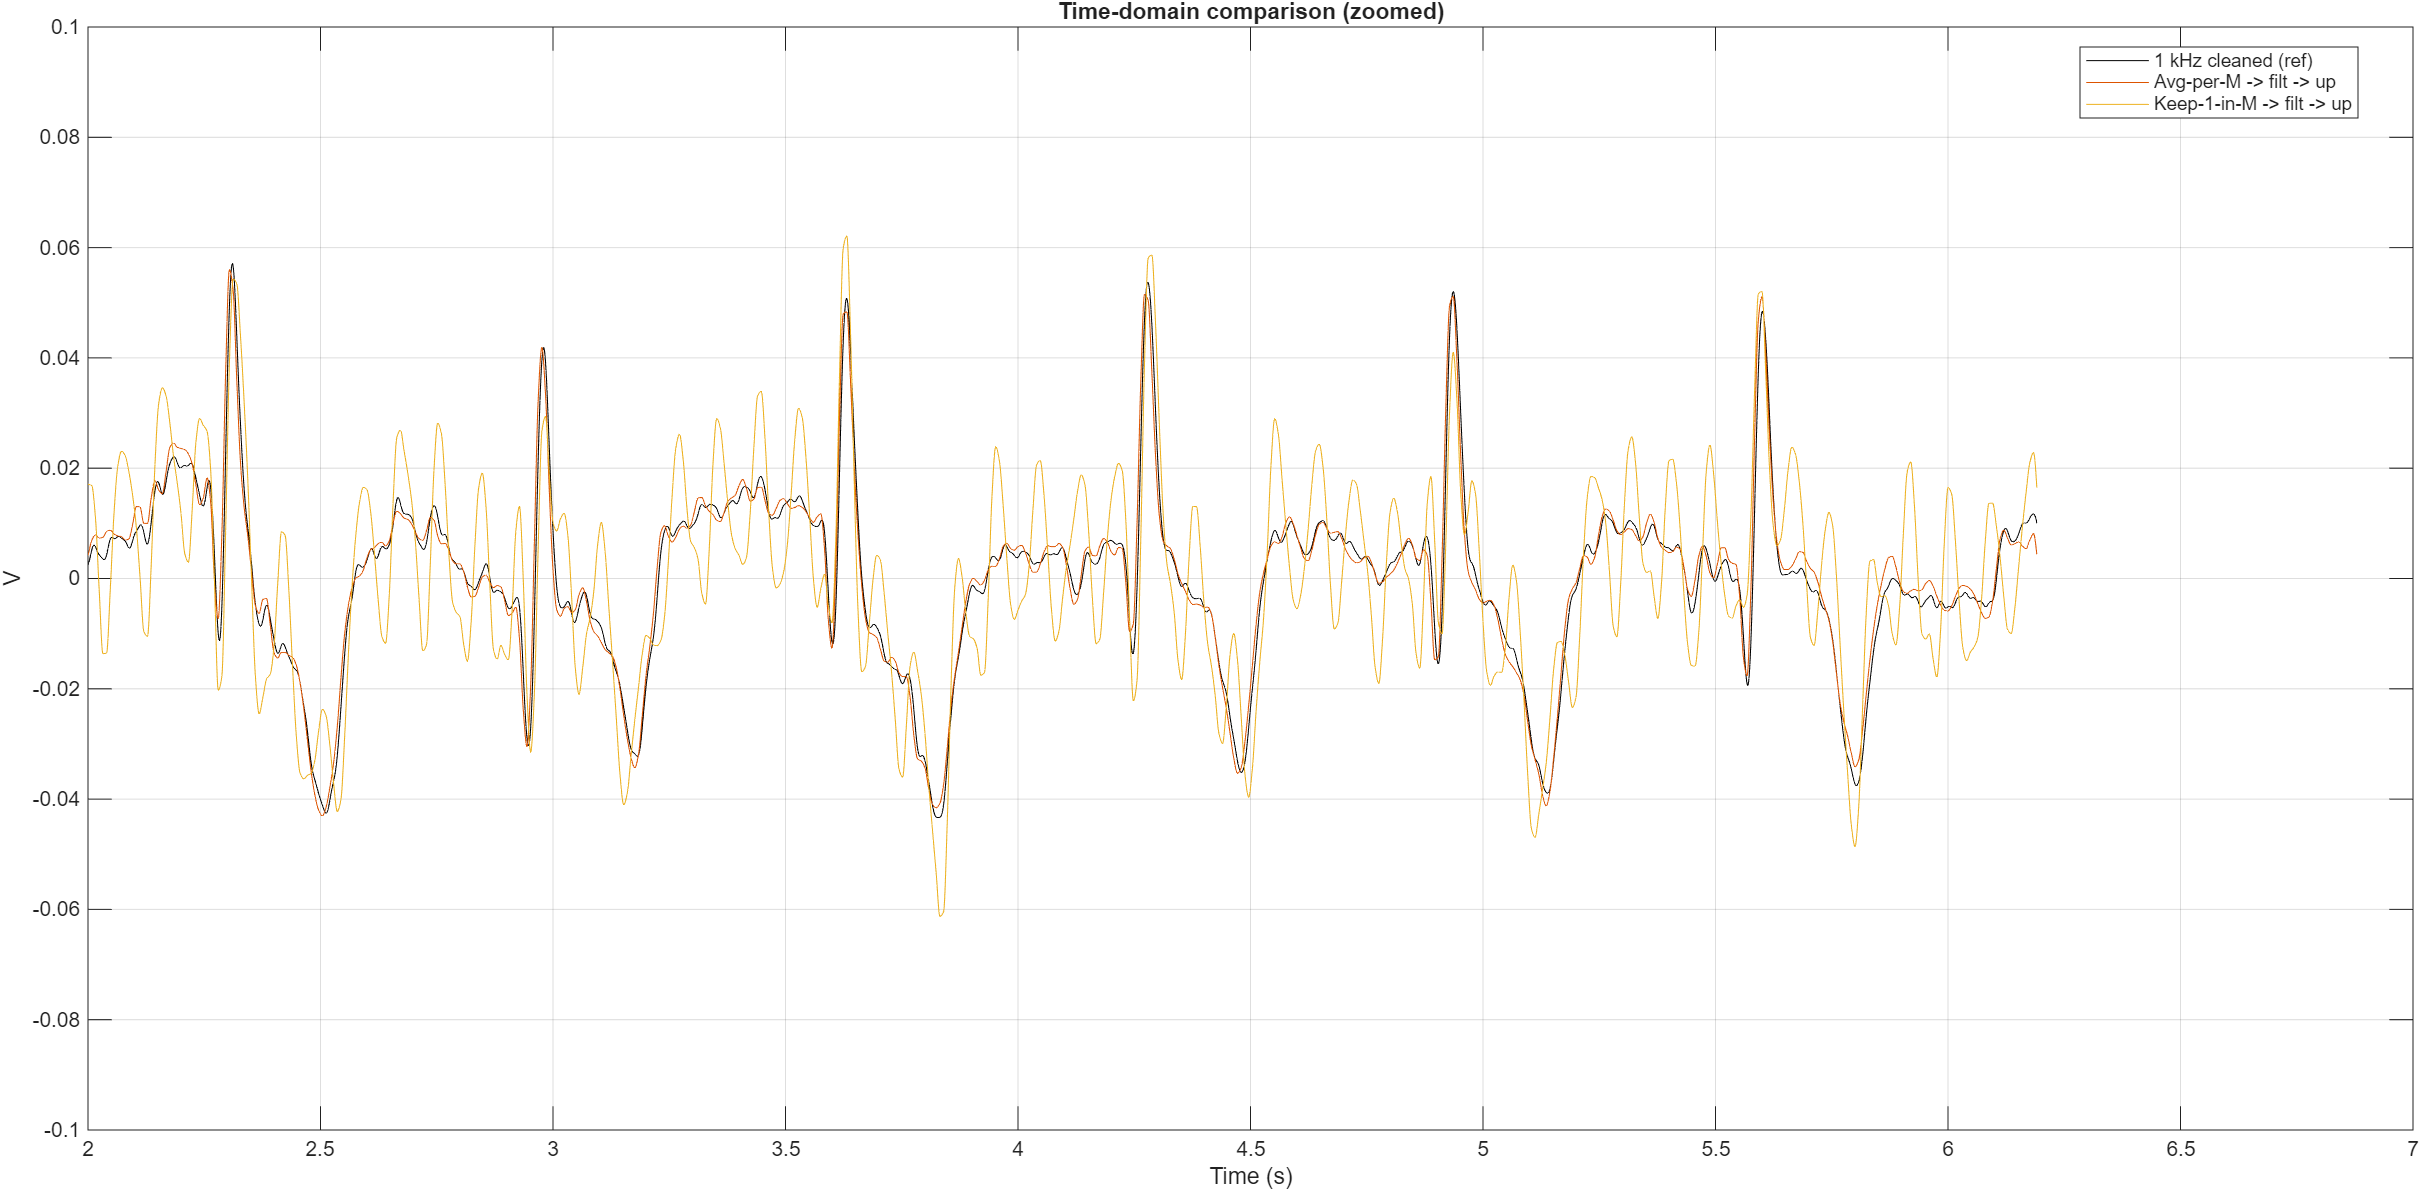
\includegraphics[width= .73\columnwidth]{fig/time_downsamp_zoom_M8.png}
    }
	\caption{Time domain signal comparison of the three different signal processing pipelines (Oversampling, Direct downsampling and Averaging downsampling)}
\label{fig:ds_time}
\end{figure}
We can observe that the downsampling signals kept more details of the ECG signals, especially obvious on the wiggles of the T peak part. 
Notice when we increase the downsample factor, the low frequency part becomes significant, and therefore the Keep-every-M design in figure \ref{fig:time_down_M8} became infeasible because it cannot effectively improve the SNR.


\subsection{Discussion on Oversampling techniques}

Oversampling in ECG acquisition serves both theoretical and practical purposes. From a signal-theoretic 
view, sampling far above the Nyquist rate does not increase the information content, but it relaxes the 
requirements on analog anti-alias filters and improves the effective resolution of quantization. In our setup, 
the ADC sampling at 1~kHz for a signal bandwidth below 30~Hz provides an oversampling ratio (OSR) of 
more than 16. Such redundancy allows digital filtering to achieve sharper cutoffs and lower in-band noise 
than a purely analog front-end could.

But the trade-offs become visible when we compare the oversampled and downsampled pipelines. 
While oversampling preserves all temporal detail and minimizes aliasing risk, it increases data volume and 
processing load. Downsampling after suitable anti-alias filtering---such as our $M=4$ and $M=8$ cases---reduces 
data rate and still maintains waveform fidelity, provided that the low-pass filter sufficiently attenuates 
frequencies above half the new sampling rate. As shown in Figure~\ref{fig:ds_freq_filt} and 
Figure~\ref{fig:ds_time}, moderate downsampling (e.g., $M=4$) preserves ECG morphology well, 
whereas overly aggressive reduction (e.g., $M=8$) leads to baseline amplification and loss of fine detail in 
the T-wave region.

From a systems perspective, this suggests that a small degree of oversampling represents 
a practical balance between SNR, computational cost, and alias-free reconstruction. In embedded ECG 
monitoring systems, this approach also allows simplified analog design: the front-end only needs a gentle 
roll-off filter, while the digital stage handles most of the noise rejection. Although oversampling may 
appear redundant at first glance, it provides robustness, flexibility in post-processing, and tolerance to 
non-ideal front-end behavior, which are key advantages for biomedical signal acquisition.


%%%%%%%%%%%%%%%%%%%%%%%%%%%%%%%%%%%%%%%%%%%%%%%%%%%%%%%%%%%%%%%%%%
\section{ECG Signal Discussion }
%%%%%%%%%%%%%%%%%%%%%%%%%%%%%%%%%%%%%%%%%%%%%%%%%%%%%%%%%%%%%%%%%%

\subsection{Our ECG Signals}

\begin{figure}[!h]
	\centering
	\subcaptionbox{\centering Eirin's ECG signal. \\$V_\text{pp} = 59$mV, BPM = $77.4$
		\label{fig:eirin}}{
		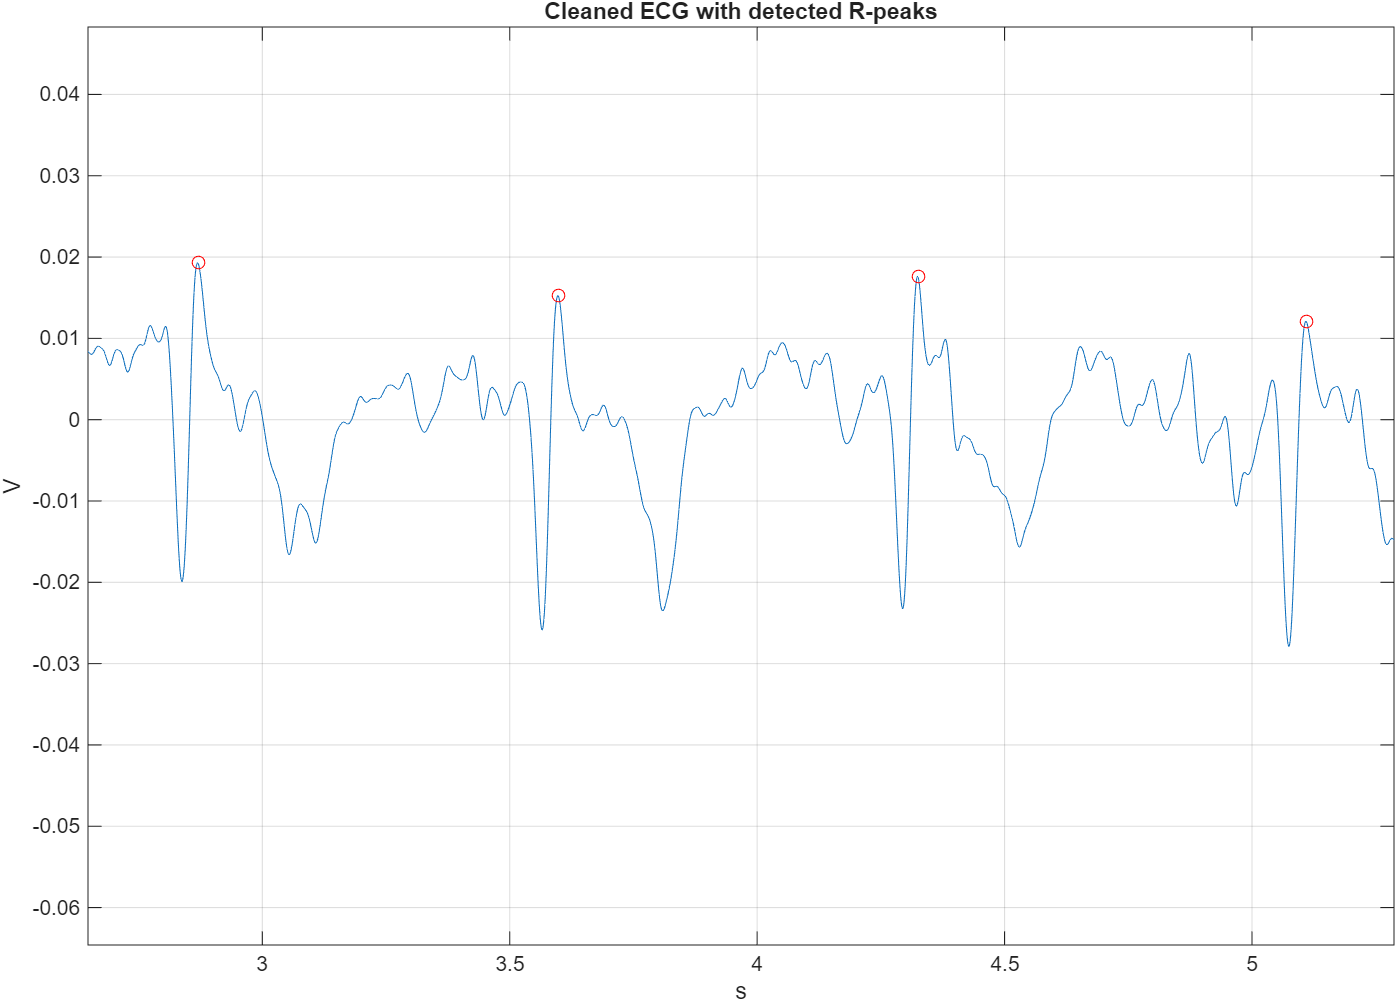
\includegraphics[width=0.31\columnwidth]{fig/eirin_77_4_0059.png}}
	\subcaptionbox{\centering Arthur's ECG signal. \\$V_\text{pp} = 44$mV, BPM = $82.2$
		\label{fig:arthur}}{
		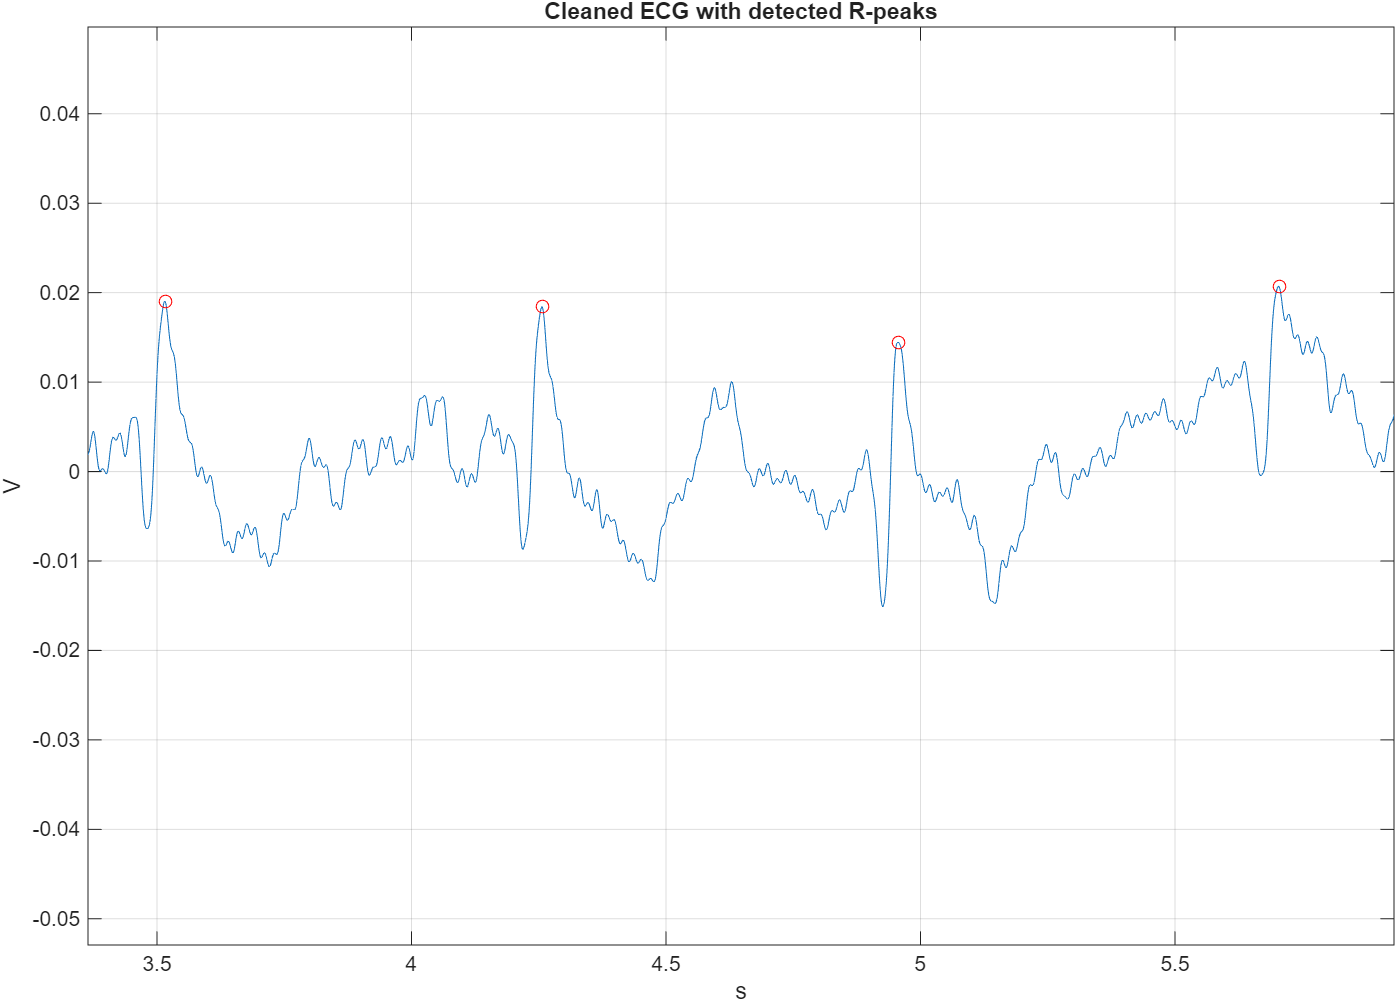
\includegraphics[width=0.31\columnwidth]{fig/arthur_82_2_0044.png}}
	\subcaptionbox{\centering Kevin's ECG signal. \\$V_\text{pp} = 100$mV, BPM = $91.2$
		\label{fig:kevin}}{
		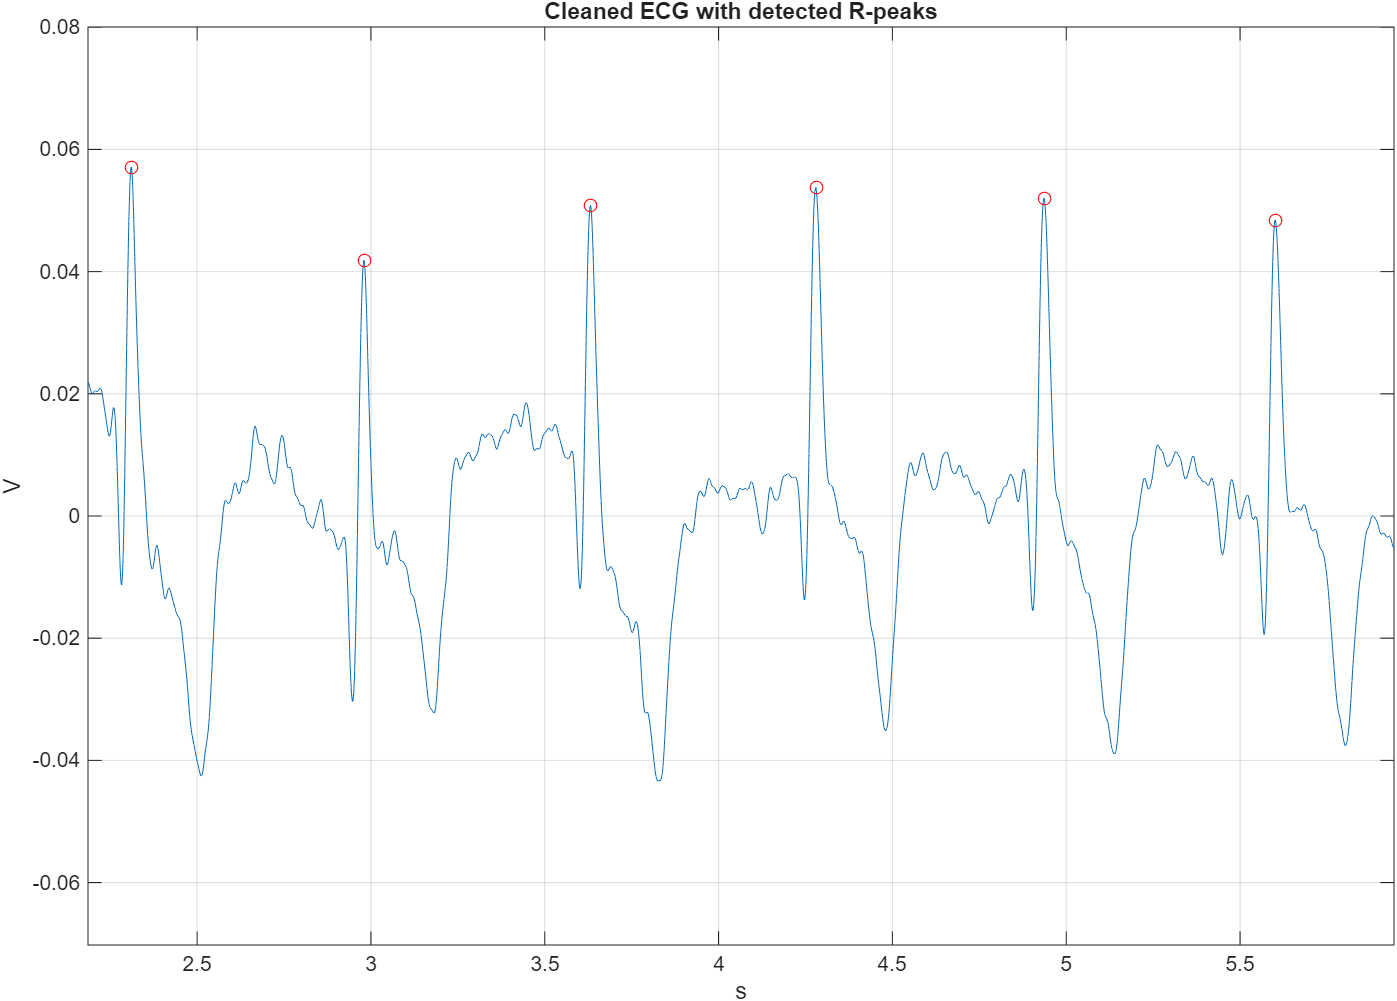
\includegraphics[width=0.31\columnwidth]{fig/kev_91_2_0100.png}}
	\caption{Our own ECG signals.}
\label{fig:real_world_image}
\end{figure}

One thing worth noticing is that Kevin is the only one in the three of us that has a regular workout habit. The signal amplitude strongly suggested that for one to improve their health they should actively consider hitting the gym more often. 

\subsection{Lead Comparison}

Based on the electrode configuration (Lead I = LA-RA, Lead II = LL-RA, Lead III = LL-LA), the recorded ECG signals show that Lead I has the largest and positive waveform, while Lead II and Lead III exhibit smaller amplitudes with inverted (negative) R-waves. This polarity difference can be explained by the relative orientation between the heart's depolarization vector and each lead's axis. When the cardiac vector points toward a lead's positive electrode, the signal appears positive; when it points away, the waveform inverts. Hence, the strong positive Lead I suggests that the heart's electrical axis was aligned closer to the LA-RA direction.

We considered both technical and physiological explanations. The literature shows that limb-lead reversal and electrode misplacement commonly produce inverted limb leads; therefore, wiring and electrode polarity should always be verified first. Instrument configuration issues—such as reversed amplifier inputs, inconsistent gain, or channel inversion—may also contribute to polarity changes.

Moreover, recent studies (The Anatolian Journal of Cardiology) indicate that electrode distance to the cardiac center correlates inversely with QRS amplitude; torso or modified limb placements can increase amplitude in certain leads. This supports the hypothesis that the closer proximity of the LA-RA electrodes to the heart could result in a larger Lead I amplitude compared with Leads II and III. In addition, environmental noise and baseline drift may further reduce the clarity of the weaker leads.

Overall, the observed differences highlight the sensitivity of ECG measurements to electrode polarity, contact quality, and spatial placement. Even small variations in electrode position or wiring can significantly alter signal polarity and amplitude.

\begin{figure}[!h]
	\centering 
		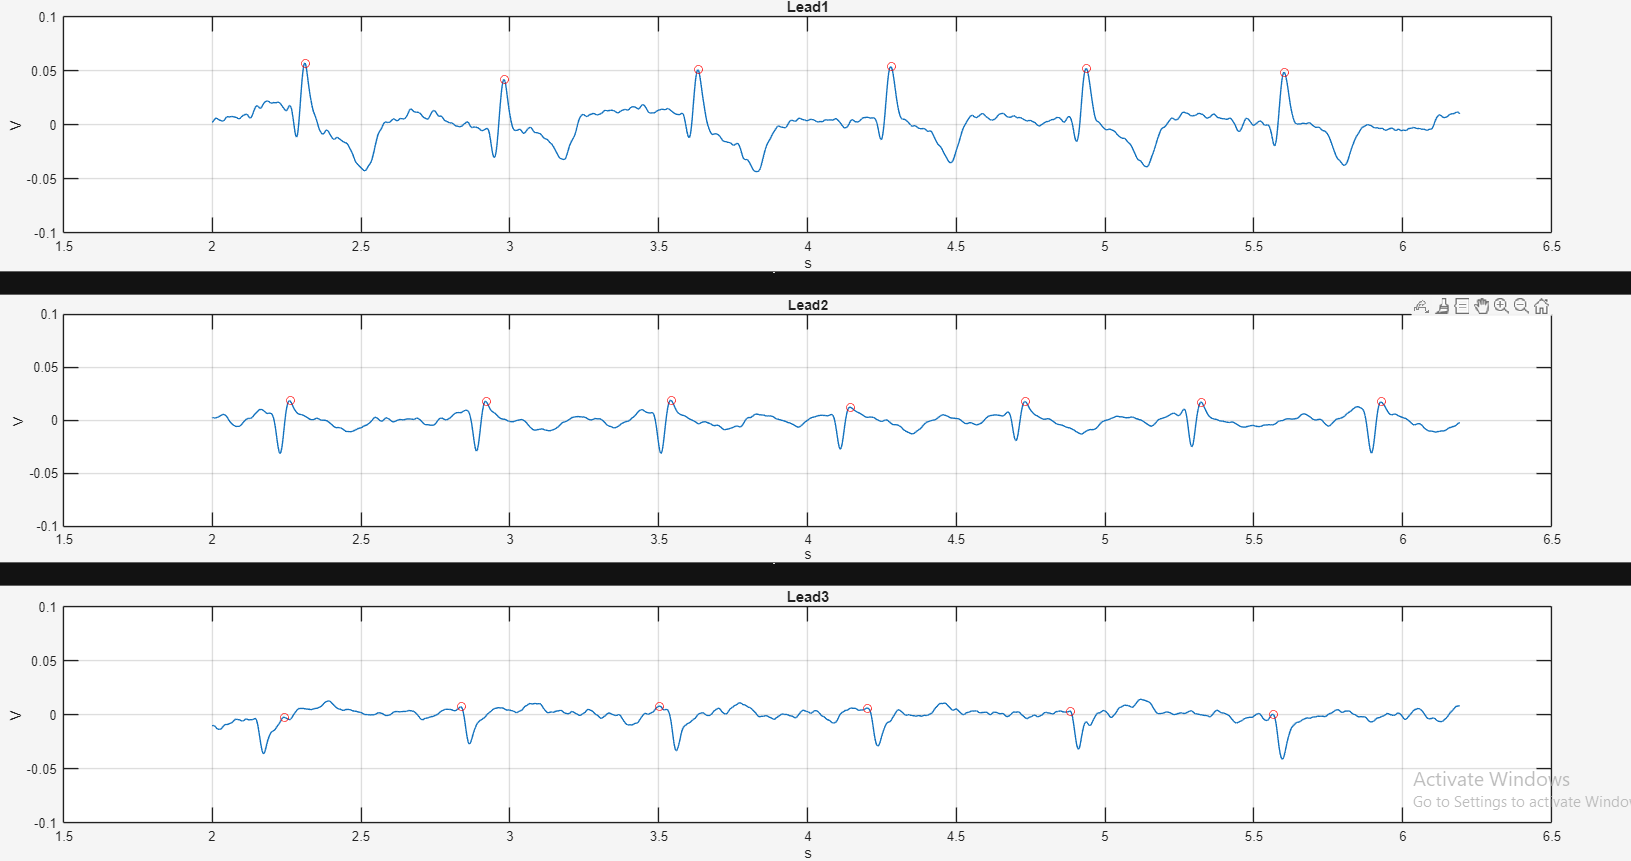
\includegraphics[width = .95\columnwidth]{fig/lead_comp.png}
	\caption{Comparing different Lead}
\label{fig:lead_time_cmp}
\end{figure}
\pagebreak

\begin{thebibliography}{99}

\bibitem{oppenheim2010dsp}
A.~V.~Oppenheim and R.~W.~Schafer,
\textit{Discrete-Time Signal Processing}, 3rd~ed.
Upper Saddle River, NJ, USA: Pearson, 2010.

\end{thebibliography}
\end{document}




